\documentclass[11pt]{scrartcl}
\usepackage{dominatrix}
\usepackage{solarized-light}
\usepackage[toc,page]{appendix}

\lstset{
language=python,
basicstyle=\ttfamily\footnotesize
}

\title{Research Summary}
\subject{Research Courses COMS W3998 and COMS W4901}
\author{Linan Qiu\\\texttt{lq2137}}
\begin{document}
\maketitle

\begin{abstract}
This report serves as a comprehensive log of what I accomplished over the two semester of research under Apoorv Agarwal and Owen Rambow. In short, I concretely defined the codeword detection problem, ran naive experiments on the problem which led to the process of systematically creating a synthetic corpus for the codeword problem, defining baseline tests, preparing datasets for such baseline tests, and finally modifying an polysemic embedding algorithm for the codeword problem. I also include extraneous results that are extensions of this main research (but do not belong to the main body of research).

This is two semester effort (Autumn 2015 and Spring 2016) for two research courses: COMS W3998 (Autumn 2015) and COMS W4901 (Spring 2016).
\end{abstract}

\newpage

\tableofcontents

\newpage

\section{Introduction}

\subsection{Problem Definition}

\subsubsection{Codewords}

I first defined codewords as words that are used differently from its ``normal'' meaning. For example, if a group of rogue traders in a bank use the word ``cheeseburger'' to denote insider information, then ``cheeseburger'' is used to in a way that is different from its usual meaning of a succulent dinner.

This problem definition can be constructed around the standard NLP literature. In the popular approach of word embeddings, the ``meaning'' of a word is usually taken to be its ``context'', or the other words that surround the given word as defined by \cite{mikolov2013distributed}. Hence, saying that ``cheeseburger'' deviates from its usual meaning under this paradigm means that in normal circumstances, ``cheeseburger'' should appear around the words ``lunch'', ``beef'' etc. while the codeword ``cheeseburger'' should appear near words like ``finance'' and ``trade''. In other words, codewords are words with contexts as they are used normally, and encoded contexts that are used by a specific group of people in a specific corpus.

\subsubsection{Communities}

Codewords also happen to be used by a subset of a population. I refer to this subset of population as a community. For example, traders committing fraud do not usually constitute the entirety of a company's employees. Instead, it is usually a single department or a select group of people within a department. Hence, codewords are also words that are used in an exclusive context by a community.

\subsubsection{Codewords in Communities}

Then, we can formally define codewords as words that

\begin{itemize}
\item possess a context that is significantly different from the context under which it is usually used
\item used by a specific community of people within a population
\end{itemize}

\subsection{Existing Work}

I started on the project in September 2015. By that time, I was fortunate to continue on the work of summer researchers under Apoorv. Specifically, I inherited the following projects.

\subsubsection{Reference Corpus}

An approach to the codeword problem is to define a reference corpus. Then, we have two corpora -- the codeword corpus $C_c$ with the codewords and the reference corpus without codewords $C_r$. For example, the codeword corpus can be the Enron corpus while the reference corpus is 20 News Group. We can generate word embeddings for both corpora and compare those embeddings to find codewords.

\subsubsection{Comparison of Cosine Distance and Matrix Distance}

Then, the summer researchers computed the cosine distances of all embeddings in both corpus: $\mathbf{V_c}$ and $\mathbf{V_r}$. Now the embedding of a given word is random, but the distribution of the entire corpus should be normal (I personally verified this hypothesis). Then, one can rotate the matrix $\mathbf{V_c}$ to match, as much as possible, $\mathbf{V_r}$ and find the outliers. These would be words that are used in a relatively different manner in both corpus. Going off the first definition of a codeword, this will be a codeword.

This measure did not produce significant results, though the matrix rotation problem in and of itself was an interesting mathematics problem. The results contained far too many false positives, and the reference corpus chosen (20 News Group) did not contain some of the codewords that were supposed to be in the Enron corpus (for example ``raptor''). This made the two difference senses (one for the original sense as a dinosaur and the other as a finance entity) undetectable.

\section{Naive Experiments}

\subsection{Naive Cosine Similarity Comparison}

The first approach I tried was to compare the cosine distance between words in the codeword corpus $C_c$ and reference corpus $C_r$. In essence, for each word $w_{i, c}$ in $C_c$, I find $w_{i, r} = w_{i, c}$ in the reference corpus and find $cossim(w_{i, c}, w_{i, r})$ for all words $i$ that are common to both corpora. The idea is that if ``hello'' is not a codeword, then $cossim(w_{hello, c}, w_{hello, r})$ should be similar to the average of all cosine similarities for all words in the corpus (\textbf{I do assume that codewords take up a very minority portion of the codeword entire vocabulary}). However, if ``cheeseburger'' is a codeword, then $cossim(w_{cheeseburger, c}, w_{cheeseburger, r})$ should be far from the mean of the cosine similarity of all words in the corpus. Then, if we plot the $cossim(w_{i, c}, w_{i, r})$ for all words $i$ in the vocabulary that is common to both corpora, then ideally I should observe a mainly normal distribution with codewords falling outside the normal distribution.

\begin{figure}[H]
\centering
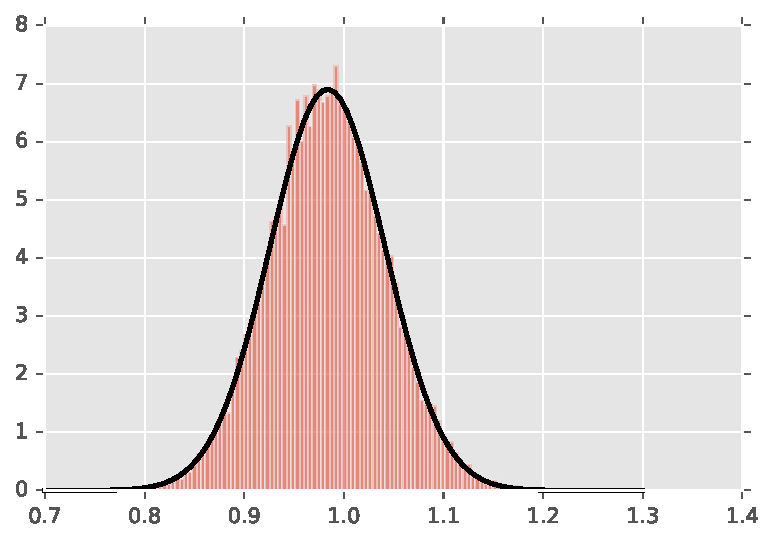
\includegraphics[width=.5\textwidth]{figures/naive-cosine-dist.pdf}
\caption{Distribution of $cossim(w_{i, c}, w_{i, r})$ for all words $i$ in the common vocabulary between $C_c$ and $C_r$ where $C_c$ is the enron corpus and $C_r$ is the 20 news group corpus}
\label{fig-naive-cosine-dist}
\end{figure}

However, this was not observed. Instead, a simple normal distribution was observed as shown in Figure \ref{fig-naive-cosine-dist}. This then required me to have a cutoff Z score for defining codewords. When I took words that are significantly different from the mean with p-value < 0.05, the words found were insignificant and unlikely to be codewords as shown in Figure \ref{fig-naive-cosine-dist-words}.

\begin{figure}[H]
foul, commented, explained, nightline, keeps, yesterday, cummings, mountains, cis, dramatically, ballistic, wishes, spi, encouraged, crash, contention, profound, interview, doubting, rudolf, slider, ray, cracking, chicken, litigation, clogged, brad, unsuccessful, champ, conclusion
\caption{A sample of words that were detected as codewords by using the p-value of 0.05 on the naive cosine distance method}
\label{fig-naive-cosine-dist-words}
\end{figure}

This method clearly did not yield codewords.

\subsection{Word Similarity Comparison}

However, the intuition behind the first method is valuable. After all, the first definition of a codeword is that it is used in a different context as it is usually used. I can approach this problem slightly different -- instead of using the embeddings of the words directly, I can ask for the similar words of a word. For example, for the word ``hello'', the words that are similar to it (i.e. the words that have the highest cosine similarity to the embedding of ``hello'') would be ``hi'', ``bye'' etc. If ``hello'' is not a codeword, we can expect this to be the same in the reference corpus. However, if ``cheeseburger'' was a codeword, the words that are similar to ``cheeseburger'' would be different in both corpus.

Formally, for a given word $w_{i, c}$ in the codeword corpus and $w_{i, r}$ in the reference corpus, we can find the set of words $\mathbf{s_{i, c}}$ that are most similar to $w_{i, c}$ and $\mathbf{s_{i ,r}}$ that are most similar to $w_{i, r}$ in the codeword corpus. I can set $|\mathbf{s_{i, c}}| = |\mathbf{s_{i, r}} = 500$. For example, this would involve me finding the 500 most similar words to ``hello'' in the codeword corpus, then the 500 most similar words to ``hello'' in the reference corpus. Then, I can calculate the intersection of these two sets $\mathbf{s_{i ,c}} \cap \mathbf{s_{i ,r}}$, and count the number of similar words that are shared in both sets (i.e. $|\mathbf{s_{i ,c}} \cap \mathbf{s_{i ,r}}|$). Intuitively, the higher this count is, the more similar the two words are used in both corpuses. Then, a codeword is simply one with a very low similarity count $|\mathbf{s_{i ,c}} \cap \mathbf{s_{i ,r}}|$.

I ran this experiment using the Enron corpus as the codeword corpus, and Wikipedia as the reference corpus. This addresses the issue of words not appearing in the reference corpus encountered earlier. The initial results were promising. For example, I know for sure that ``good'', ``finance'', and ``meeting'' are not codewords in the Enron corpus. These words had similarity counts of 142, 75, and 54 respectively. I also know that ``raptor'' is a codeword in Enron. The similarity count for ``raptor'' is 2.

At this point, before testing the results further, Apoorv and I realized that we needed to find a way to systematically test our results. We needed a synthetic codeword dataset that reflects our definitions of codewords. This can then be used to systematically test our results.

\section{Synthetic Corpus}

No dataset specifically containing a known list of codewords in the way I defined exists. This frustrates research efforts since a dataset is needed to establish baselines and run experiments. Hence, I created a synthetic dataset for this problem.

\subsection{Approach Overview}

\subsubsection{Easy Codeword Corpus}

The general idea is to generate a synthetic codeword corpus $C_c$ from a reference corpus $C_r$. By creating a few codewords in a corpus known not to have many codewords, this method allows me to test codeword detection against the synthetic codewords. The steps are:

\begin{itemize}
\item Get a reference corpus containing little to no codewords (e.g. the WSJ corpus)
\item Select $n$ words in the corpus.
\item For each of these $n$ words (i.e. $w_{i, r}$ for all $i \in 1 ... n$), generate a set of words $w_{j, r}$ where $w_{i, r} \neq w_{j, r}$ for $j \in 1 .. n$. In other words, map each word select to another word in the set of $n$ words.
\item Generate a codeword corpus by replacing all $w_{i, r}$ with $w_{j, r}$.
\end{itemize}

For example, if I select the words ``hello'', ``cheeseburger'', and ``fruit'' in the reference corpus, then ``hello'' could be replaced by ``cheeseburger'', ``cheeseburger'' replaced by ``fruit'', and ``fruit'' replaced by ``hello''. This means that in the synthetic codeword corpus, I would see the sentence ``cheeseburger, have a good day'' instead of ``hello, have a good day''. This captures the first semantic of a codeword: a word being used in a context different than its usual context. In the synthetic corpus, I have created an extreme example -- compared to the reference corpus, all contexts of ``hello'' has been modified to that of ``cheeseburger''s.

\subsubsection{Hard Codeword Corpus}

Alternatively, a ``harder'' codeword corpus can be generated. This captures both semantics of codewords -- both different contexts and specific subgroups of users.

\begin{itemize}
\item Get a reference corpus containing little to no codewords (e.g. the WSJ corpus)
\item Select $n$ words in the corpus.
\item For each of these $n$ words (i.e. $w_{i, r}$ for all $i \in 1 ... n$), generate a set of words $w_{j, r}$ where $w_{i, r} \neq w_{j, r}$ for $j \in 1 .. n$. In other words, map each word select to another word in the set of $n$ words.
\item Generate a codeword corpus by replacing all $w_{i, r}$ with $w_{j, r}$ \textbf{within a specific subset (community) of documents}.
\end{itemize}

For this harder approach, one could imagine an already partitioned corpus (such as Reddit, where each forum (subreddit) is grouped into a single community). Then, replacements are only done to words in a community, but not to words outside those community. Hence, ``hello'' will be replaced by ``cheeseburger'' only within, say, the \texttt{/r/gaming} community, but not in everything else.

There are two problems to tackle:

\begin{enumerate}
\item What reference corpus should I use to generate the synthetic corpus from
\item How do I select salient, important words to be used as codewords (not words such as ``the'' and ``he''
\end{enumerate}

These will be addressed in the next section.

\subsection{Reference Corpus choice}

I choose the WSJ Corpus from the PennTreebank to be the reference corpus due to the similarity in the content of the text and the data of potential clients. A helper function is made in \lstinline{lib.corpus_parser} to use \lstinline{nltk} to parse the WSJ corpus. Tip to future replications: use a symlink to link \lstinline{LDC99T42-Treebank-3/package/treebank 3/parsed/mrg/wsj} and \lstinline{LDC99T42-Treebank-3/package/treebank 3/parsed/mrg/brown} to \lstinline{~/nltk data/corpora/ptb/wsj} and \lstinline{~/nltk data/corpora/ptb/brown} so that \lstinline{nltk} can parse the WSJ corpus directly.

For the harder codeword corpus, I used a Reddit dataset scraped from Reddit using a scraper I wrote (\url{github.com/linanqiu/omega-red}). Details of this project is left in the appendix. The advantage of this corpus is that I am able to obtain pre-labeled communities. Reddit forums exist in the form of subreddits and metareddits. Subreddits are individual forums related to a topic, such as football or baseball. Metareddits are groupings of subreddits around a theme, such as news, politics, sports etc. My scraper obtained 5000 threads from each of the following subreddits in each of the following metareddits.

\begin{figure}[h]
\begin{itemize}
\item[news]: politics, worldnews, news, conspiracy, libertarian, truereddit, conservative, offbeat
\item[lifestyle]: food, guns, motorcycles, sex, progresspics, lifehacks, frugal, drunk
\item[learning]: todayilearned, science, askscience, space, askhistorians, youshouldknown, explainlikeimfive
\item[humor]: funny, adviceanimals, imgoingtohellforthis, facepalm, jokes, circlejerk
\item[entertainment]: music, movies, harrypotter, starwars, anime, comicbooks
\item[television]: gameofthrones, doctorwho, mylittlepony, community, breakingbad, startrek, himym, thewalkingdead
\item[gaming]: gaming, leagueoflegends, pokemon, minecraft, starcraft, dota2, skyrim, tf2
\end{itemize}
\caption{Listing of metareddits and subreddits in the reddit corpus. 5000 threads and comments were scraped from each subreddit.}
\label{fig-reddit-corpus}
\end{figure}

As shown in Figure \ref{fig-reddit-corpus}, I obtained a total of 800MB of Reddit data.

\subsection{Selecting Salient Words}

I also needed a way to select $n$ codewords (in this case I used $n = 100$ in most corpus based on intuition about the size of the corpus and usage patterns)

\subsubsection{TF-IDF}

A naive way to do this would be TF-IDF. I used this initially, where

\begin{itemize}
\item $T_{i, r}$ is the number of times word $w_{i, r}$ appeared in the corpus $C_r$
\item $D_{i, r}$ is the number of documents (in the case of WSJ, separate articles) that word $w_{i, r}$ appeared in
\item $N_D$ is the number of documents in the entire corpus
\end{itemize}

Then, each word is assigned a rank $R_{i, r}$ where

\[R_{i, r} = TFIDF_{i, r} = \log{\left(T_{i, r} + 1\right)} * \log{\left(1 + \frac{N_D}{D_{i, r}}\right)}\]

The left term is the term frequency smoothed so that 0s won't occur, and the right term is the inverse document frequency.

We select the top $n$ words with the highest $R_{i, r}$. The intuition behind this method was to downweight terms that appeared in every document (such as ``the'', ``a'', ``he''), and upweight rarer terms.

However, this method was disappointing since it upweighted rare terms too much. In particular, note that the inverse document frequency portion of TFIDF is a decreasing function. That means words appearing only 1 time is upweighted the most. Hence, a lot of names and esoteric words that only occur once were selected. The top words consisted of ``yeargin'', ``steinhardt'', ``corry'', ``psyllium''. We needed an alternative method that downweighted very frequent words, upweighted rarer words, but also downweighted extremely rare words.

\subsubsection{Gamma Weighted TF-IDF}

Instead, I discovered that a good way to do this was to use a Gamma distribution instead of the inverse document frequency measure. That means 

\[R_{i,r} = \log{\left(T_{i, r} + 1\right)} * g\left(D_{i, r}\right)\]

where $g(y)$ is the Gamma distribution function fitted on a given $\alpha$ and $\beta$. Specifically, I can set $\alpha$ and $\beta$ such that the mode of the distribution is a certain proportion of documents (i.e. this is the proportion of documents that ``important words'' should belong in) and the mean to be 2 times of that. Choosing $mode = 0.075*N_D = (\alpha - 1) * \beta$ and hence $mean = 0.15 * N_D = \alpha * \beta$ we make the assumption that important words should be present in around 7.5\% to 15\% of articles. The gamma distribution hence looks like Figure \ref{fig-gamma-dist}.

\begin{figure}[h]
\centering
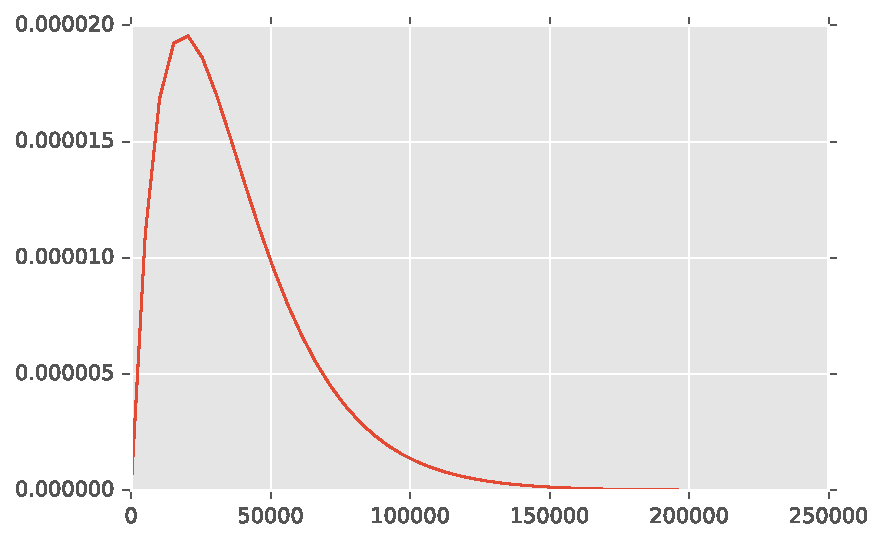
\includegraphics[width=.5\textwidth]{figures/gamma-dist.pdf}
\caption{Gamma distribution $g(x)$ used to upweight important words.}
\label{fig-gamma-dist}
\end{figure}

This function upweights words that appear not so frequently, but downweights words that appear very rarely (along with words that appear frequently). The results turned out to be very reasonable for the WSJ corpus. Top words include ``bonds'', ``index'', ``japanese'', ``oil'', ``traders''.

This result should not be surprising given that TF-IDF is a measure meant for weighting words in a single document among many documents, not an aggregate measure across documents.
This allows us to select $n$ words by taking the top $n = 100$ words using $R_{i,r}$

\subsection{Generating a Substitute Corpus}

Now that I have selected the most salient $n$ words in a corpus, I want to create a matching between $w_{i, r}$ and $w_{j, r}$ as mentioned earlier. This matching should be such that $w_{i, r} \neq w_{j, r}$ for all $i$ and $j$ in $1 ... n$. This is rather trivial, and we simply shuffle the set of $n$ words to get $j$.

Then, we can generate a codeword corpus by going through the reference corpus and replacing every occurrence of word $w_{i, r}$ with $w_{j, r}$.

We generated the following easy and hard synthetic codeword corpora:

\begin{itemize}
\item (Easy) WSJ synthetic corpus generated by replacing 100 words in the entire WSJ corpus
\item (Easy) Reddit synthetic corpus generated by replacing 100 words in the entire reddit corpus
\item (Hard) 7 Reddit community synthetic corpus generated by replacing 100 words in only 1 metareddit (community) of the reddit corpus while leaving the rest of the corpus in tact
\end{itemize}

\section{Word Similarity Approach}

\subsection{Results using Word2Vec on Synthetic WSJ Corpus with Reference WSJ Corpus}

Recall the earlier definition of the word similarity metric $|\mathbf{s_{i ,c}} \cap \mathbf{s_{i ,r}}|$ where $C_c$ is the synthetic WSJ corpus and $C_r$ is the original WSJ corpus. I can now detect codewords by setting a threshold tolerance $x$ on the word similarity metric; I can declare a word $i$ as a codeword if $|\mathbf{s_{i ,c}} \cap \mathbf{s_{i ,r}}| < x$.

I first use this approach on the synthetic WSJ corpus generated by replacing \textbf{all} 100 selected words in the WSJ corpus. Note that this only takes into account the first definition of codeword regarding different contexts. Embeddings for each of the corpora is generated using Word2Vec's Skip-gram with negative sampling algorithm. In other words, we generate

\begin{itemize}
\item Embedding $E_{i, c}$ for each word $w_{i, c}$ in the synthetic WSJ corpus
\item Embedding $E_{i, r}$ for each word $w_{i, r}$ in the reference WSJ corpus
\end{itemize}

The two embeddings are generated \textbf{separately} since I want to know the different contexts of both corpora.

As shown in Figure \ref{fig-wsj-count}, synthetic codewords are well captured and the differing context of the substituted words are caught. Codewords have significantly lower $x$ than non codewords. Figure \ref{fig-wsj-f1} shows high precision, recall, and F1 score for this experiment.

\begin{figure}[h]
\centering
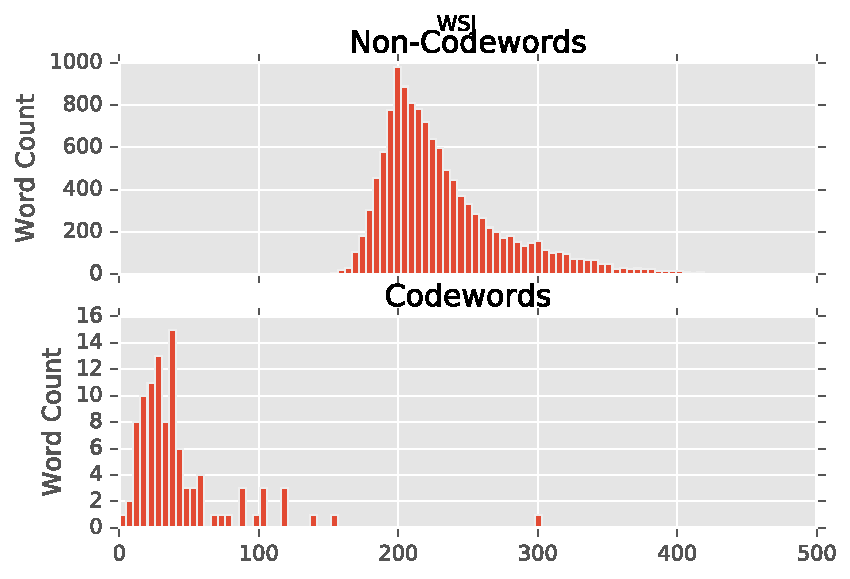
\includegraphics[width=.5\textwidth]{figures/wsj-count.pdf}
\caption{$x$ for non-codewords and codewords generated for every word $w_{i, c}$ and $w_{i, r}$, with $C_c$ being the synthetic WSJ corpus and $C_r$ being the original WSJ corpus. Synthetic codewords are well captured and the differing context of the substituted words are caught. Codewords have significantly lower $x$ than non codewords.}
\label{fig-wsj-count}
\end{figure}

\begin{figure}[h]
\centering
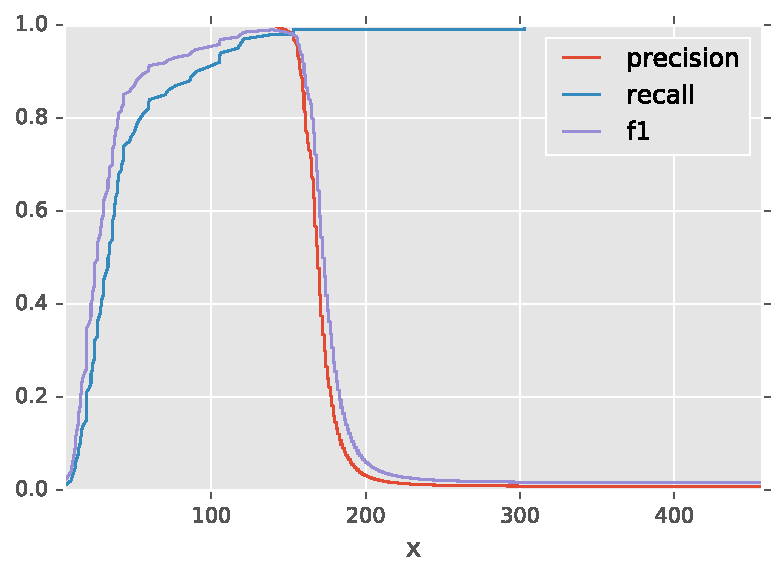
\includegraphics[width=.5\textwidth]{figures/wsj-f1.pdf}
\caption{The precision, recall, and F1 score of codeword detection for $C_c$ being the synthetic WSJ corpus and $C_r$ being the original WSJ corpus}
\label{fig-wsj-f1}
\end{figure}

This experiments represents a highly idealized scenario where

\begin{itemize}
\item I have an exact reference corpus available with the same vocabulary and general language pattern. This is implied by the use of the WSJ corpus as reference corpus (against the synthetic WSJ corpus). A more realistic scenario would be using the Wikipedia corpus or another corpus as the reference corpus against the synthetic WSJ corpus.
\item Codewords are used by the entire population. This is implied by the full substitution process (where every single document in the corpus has codewords substituted).
\item A codeword is never used in another context. For example, if ``cheeseburger'' was a codeword that denotes financial fraud, it is never used to denote the food. This is implied by the substitution process.
\end{itemize}

I can break down these assumptions to see how the embedding + word similarity method performs.

\subsection{Results using Word2Vec on Synthetic WSJ Corpus with External Reference Corpus}

One of the advantages of the word similarity method is that I am not limited by the format of the embeddings. That is, the codeword corpus and the reference corpus do not need to have the same dimensions of embeddings (unlike if I did the original method of cosine matrix rotation). This allows me to use external, pre-trained corpora. Hence, instead of the original WSJ reference corpus, I used Google News and Wikipedia (separately) as reference corpus. Under these (uncleaned and rather different) corpora, the word similarity method performed a lot poorer.

\subsubsection{Google News as Reference Corpus}

I first used the pre-trained Google News corpus available at \url{https://code.google.com/archive/p/word2vec/}. The results were significantly worse than the one using WSJ as the reference corpus.

\begin{figure}[h]
\centering
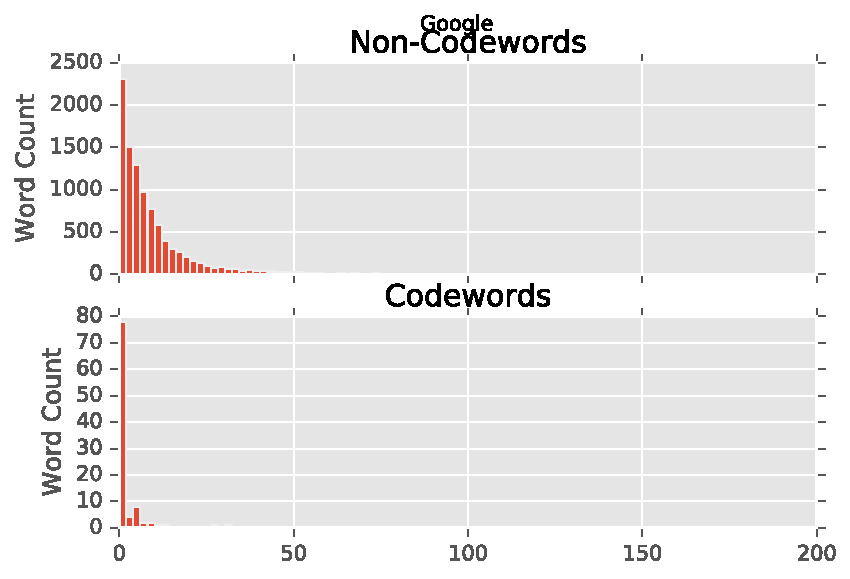
\includegraphics[width=.5\textwidth]{figures/google-count.pdf}
\caption{$x$ for non-codewords and codewords generated for every word $w_{i, c}$ and $w_{i, r}$, with $C_c$ being the synthetic WSJ corpus and $C_r$ being the Google News corpus. Non-codewords and codewords alike have low $x$, even though non-codewords have a higher tail. This results in the high false positive as can be seen in Figure \ref{fig-google-f1}}
\label{fig-google-count}
\end{figure}

\begin{figure}[h]
\centering
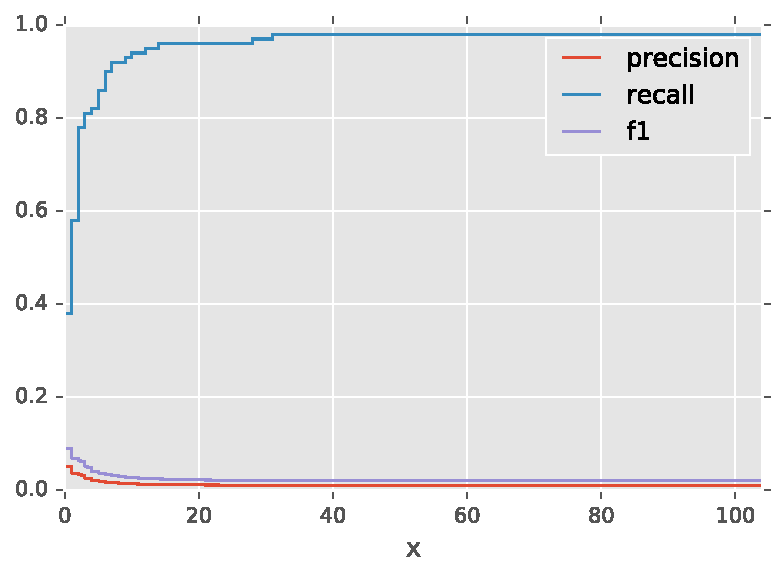
\includegraphics[width=.5\textwidth]{figures/google-f1.pdf}
\caption{The precision, recall, and F1 score of codeword detection for $C_c$ being the synthetic WSJ corpus and $C_r$ being the Google News corpus.}
\label{fig-google-f1}
\end{figure}

I observed a high false positive rate. Non-codewords and codewords alike have low $x$, even though non-codewords have a higher tail. This results in the high false positive as can be seen in Figure \ref{fig-google-f1}.

\subsubsection{Wikipedia as Reference Corpus}

I also used the Wikipedia word2vec corpus available at \url{http://textminingonline.com/training-word2vec-model-on-english-wikipedia-by-gensim}. The results were again significantly worse.

\begin{figure}[h]
\centering
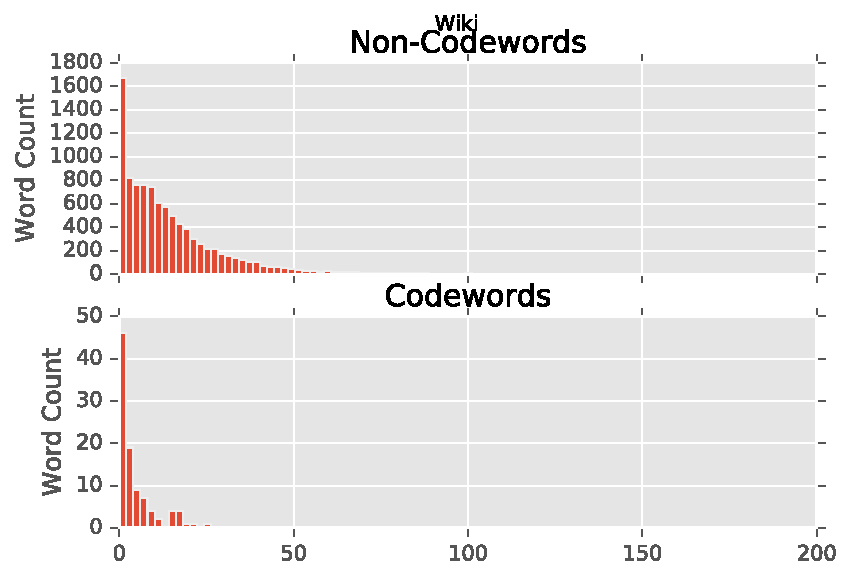
\includegraphics[width=.5\textwidth]{figures/wiki-count.pdf}
\caption{$x$ for non-codewords and codewords generated for every word $w_{i, c}$ and $w_{i, r}$, with $C_c$ being the synthetic WSJ corpus and $C_r$ being the Wikipedia corpus. Non-codewords and codewords alike have low $x$, even though non-codewords have a higher tail. This results in the high false positive as can be seen in Figure \ref{fig-wiki-f1}}
\label{fig-wiki-count}
\end{figure}

\begin{figure}[h]
\centering
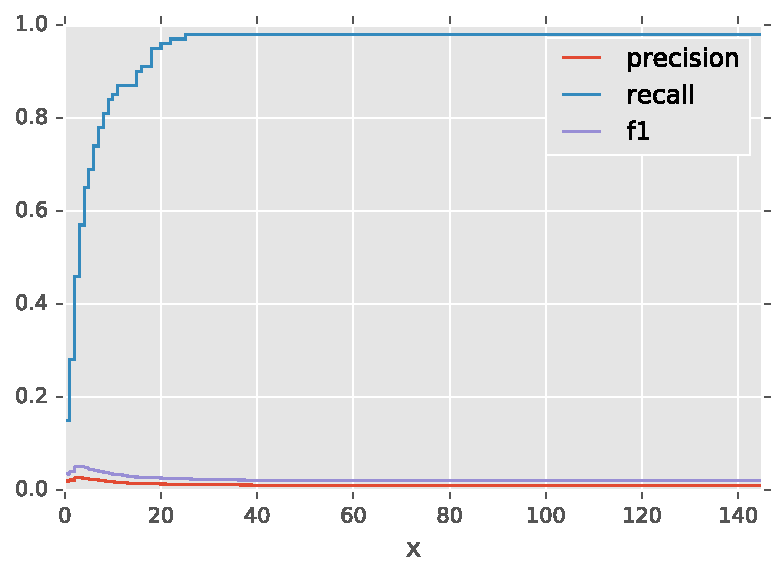
\includegraphics[width=.5\textwidth]{figures/wiki-f1.pdf}
\caption{The precision, recall, and F1 score of codeword detection for $C_c$ being the synthetic WSJ corpus and $C_r$ being the Wikipedia corpus.}
\label{fig-wiki-f1}
\end{figure}

I again observed a high false positive rate. Non-codewords and codewords alike have low $x$, even though non-codewords have a higher tail. This results in the high false positive as can be seen in Figure \ref{fig-wiki-f1}.

This shows that simply using a random external corpus, while intuitively correct, does not produce sufficiently good results due to a large amount of noise. Hence, the choice of reference corpus matters significantly in producing good results.

\subsection{Results using Word2Vec on Synthetic Reddit Corpus with Reddit Reference Corpus}

Next, I test the robustness of this algorithm against the second definition codewords -- that only a small subset of the population (a community) uses the codeword.

\subsubsection{Entire Reddit Corpus}

First, I run an experiment using the easy synthetic Reddit codeword corpus. This is the one with all instances of codewords substituted in the entire corpus (in all 7 communities). In other words, I am simply using a noisier corpus (Reddit) instead of WSJ. This is compared against the original Reddit reference corpus.

\begin{figure}[h]
\centering
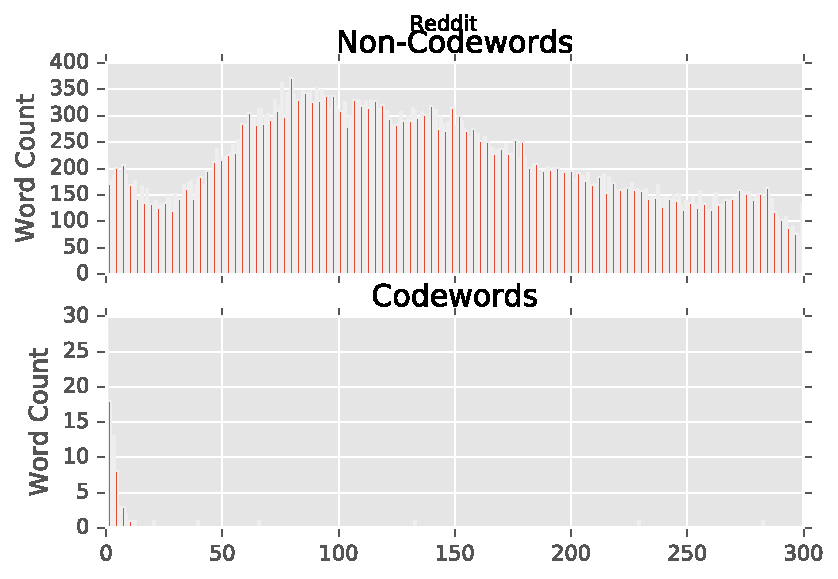
\includegraphics[width=.5\textwidth]{figures/reddit-count.pdf}
\caption{$x$ for non-codewords and codewords generated for every word $w_{i, c}$ and $w_{i, r}$, with $C_c$ being the synthetic Reddit corpus and $C_r$ being the original Reddit corpus. Codewords have significantly lower $x$ than non-codewords. However, the standard deviation of the non-codeword distribution is much fatter, resulting in a higher false positive rate as shown in Figure \ref{fig-reddit-f1}}
\label{fig-reddit-count}
\end{figure}

\begin{figure}[h]
\centering
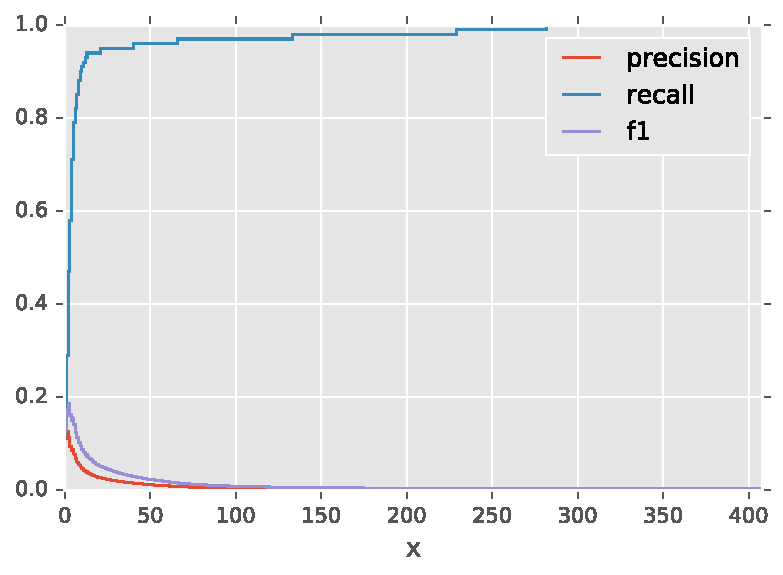
\includegraphics[width=.5\textwidth]{figures/reddit-f1.pdf}
\caption{The precision, recall, and F1 score of codeword detection for $C_c$ being the synthetic Reddit corpus and $C_r$ being the original Reddit corpus.}
\label{fig-reddit-f1}
\end{figure}

I find that performance degrades. Codewords have significantly lower $x$ than non-codewords. However, the standard deviation of the non-codeword distribution is much fatter, resulting in a higher false positive rate as shown in Figure \ref{fig-reddit-f1}. However, we are still able to recall around 80\% of codewords while maintaining a rather low precision and F1 score. This can be attributed to the noise of the Reddit corpus.

\subsubsection{Introducing Communities}

To simulate communities, only 1 of the 7 communities in each of the 7 hard reddit synthetic corpora have substitutions. In other words, for the corpus where the ``humor'' community is defined to have codewords, codeword substitutions are only performed within the portion of the corpus belonging to the ``humor'' metareddit. For example, if the ``hello'' to ``cheeseburger'' substitution is performed, it will only be performed within the ``humor'' community. All the others (``entertainment'', ``gaming'', ``learning'', ``lifestyle'', ``news'', ``television'') do not contain the substitutions.

As shown in Figure \ref{fig-reddit-community-count} and \ref{fig-reddit-community-f1}, the embedding + word similarity method performed significantly worse. There was almost no distinction between codewords and non-codewords.

One reason may be that the Reddit corpus is noisier. However, as I have shown in the earlier experiment involving the \textbf{entire} Reddit corpus, the results from a noisy corpus is still somewhat decent. The more important reason is that of the embedding method I used. Word2Vec assigns a single embedding to each word $i$: $w_{i, r}$ or $w_{i, c}$ in codeword corpus or the reference corpus accordingly. In doing so, this usage assumes that all codewords (e.g. all instances of ``cheeseburger'') are used only in the context of the codeword and not in the original sense. However, if there were \textbf{both} people using ``cheeseburger'' in the sense of the food, and in its codeword context as a fraudulent activity, then a single embedding cannot capture these two different senses. Instead, the embedding would be an average of the two, making no sense whatsoever.

\begin{figure}[H]
\begin{subfigure}[t]{.4\textwidth}
\centering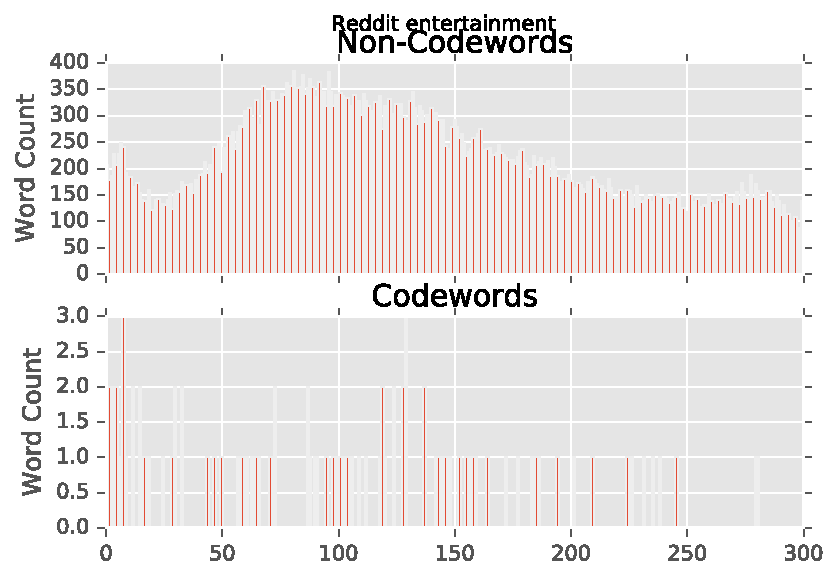
\includegraphics[]{figures/reddit-entertainment-count.pdf}
\caption{``entertainment''}
\label{fig-reddit-entertainment-count}
\end{subfigure}
\begin{subfigure}[t]{.4\textwidth}
\centering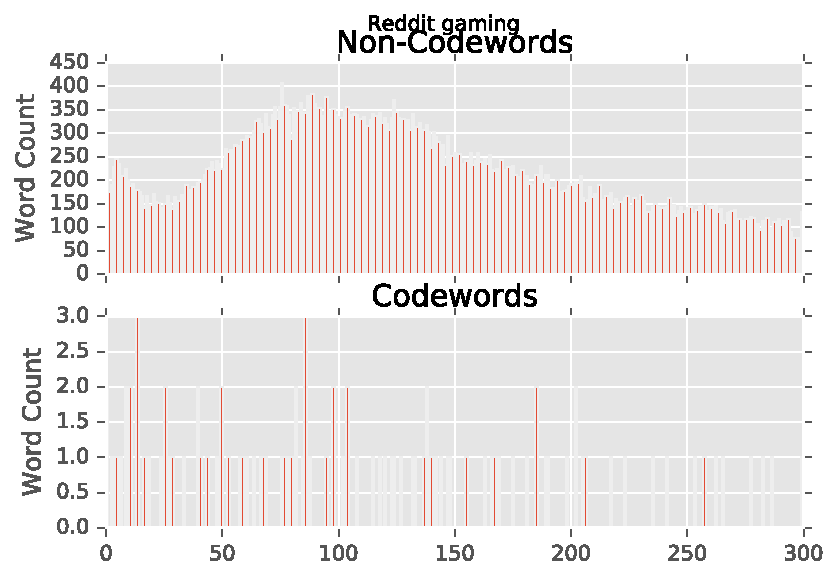
\includegraphics[]{figures/reddit-gaming-count.pdf}
\caption{``gaming''}
\label{fig-reddit-gaming-count}
\end{subfigure}
\begin{subfigure}[t]{.4\textwidth}
\centering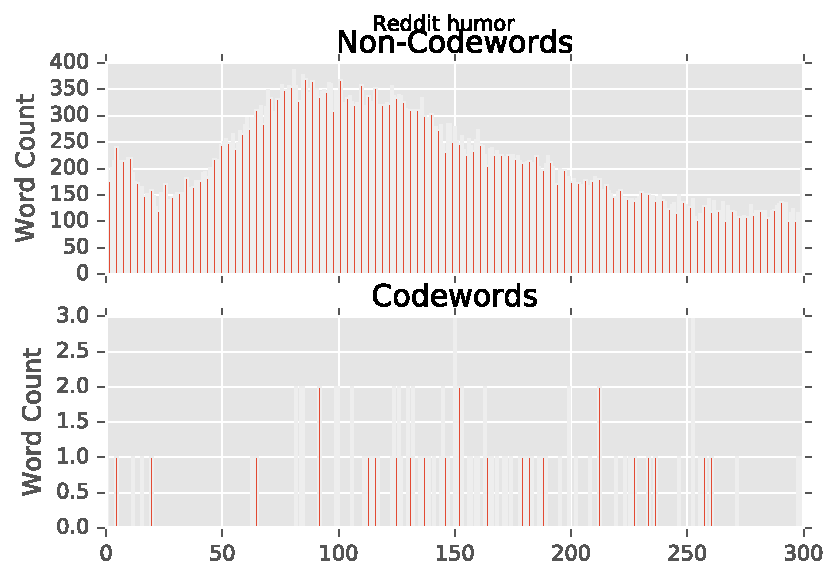
\includegraphics[]{figures/reddit-humor-count.pdf}
\caption{``humor''}
\label{fig-reddit-humor-count}
\end{subfigure}
\begin{subfigure}[t]{.4\textwidth}
\centering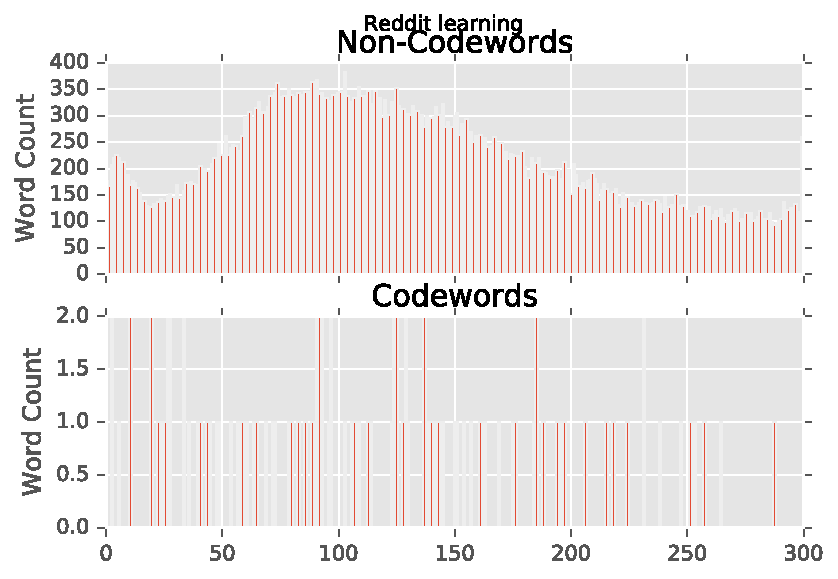
\includegraphics[]{figures/reddit-learning-count.pdf}
\caption{``learning''}
\label{fig-reddit-learning-count}
\end{subfigure}
\begin{subfigure}[t]{.4\textwidth}
\centering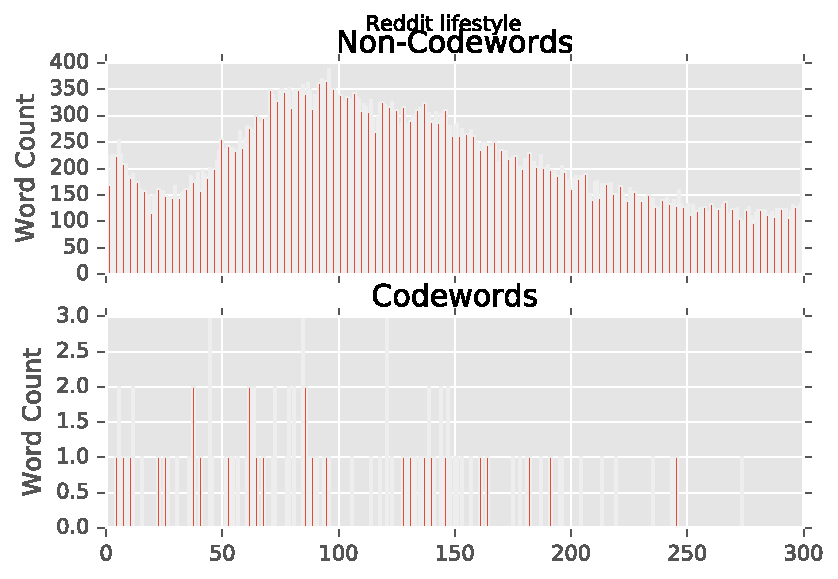
\includegraphics[]{figures/reddit-lifestyle-count.pdf}
\caption{``lifestyle''}
\label{fig-reddit-lifestyle-count}
\end{subfigure}
\begin{subfigure}[t]{.4\textwidth}
\centering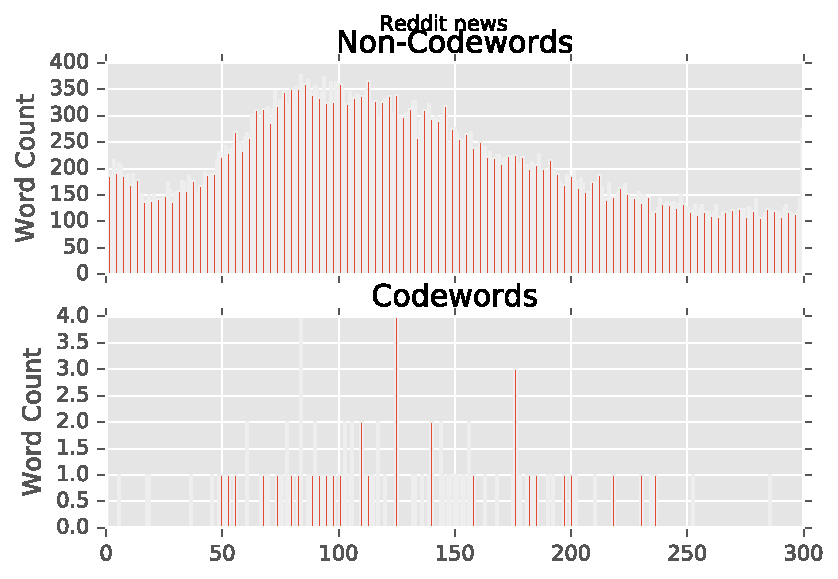
\includegraphics[]{figures/reddit-news-count.pdf}
\caption{``news''}
\label{fig-reddit-news-count}
\end{subfigure}
\begin{subfigure}[t]{.4\textwidth}
\centering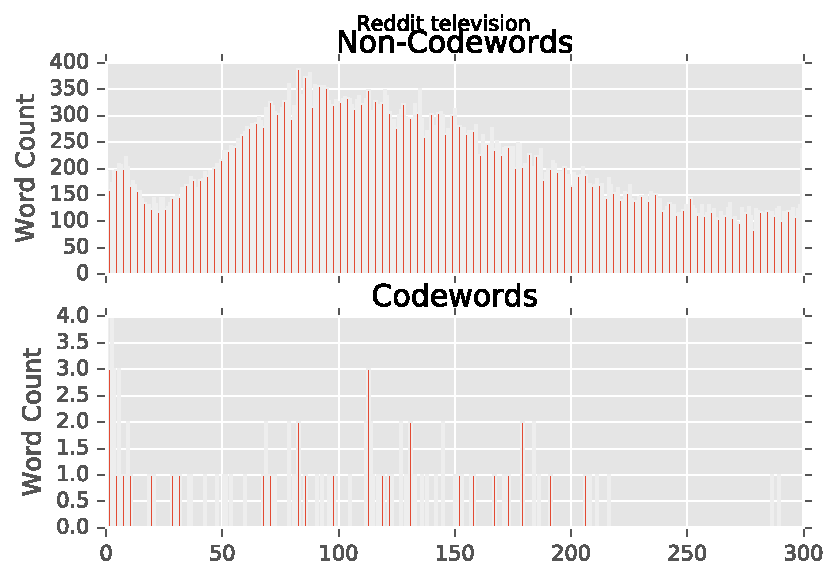
\includegraphics[]{figures/reddit-television-count.pdf}
\caption{``television''}
\label{fig-reddit-television-count}
\end{subfigure}
\caption{$x$ for non-codewords and codewords generated for every word $w_{i, c}$ and $w_{i, r}$, with $C_c$ being the hard synthetic Reddit corpus (codewords only in one of the communities) and $C_r$ being the original Reddit corpus.}
\label{fig-reddit-community-count}
\end{figure}

\begin{figure}[H]
\begin{subfigure}[t]{.4\textwidth}
\centering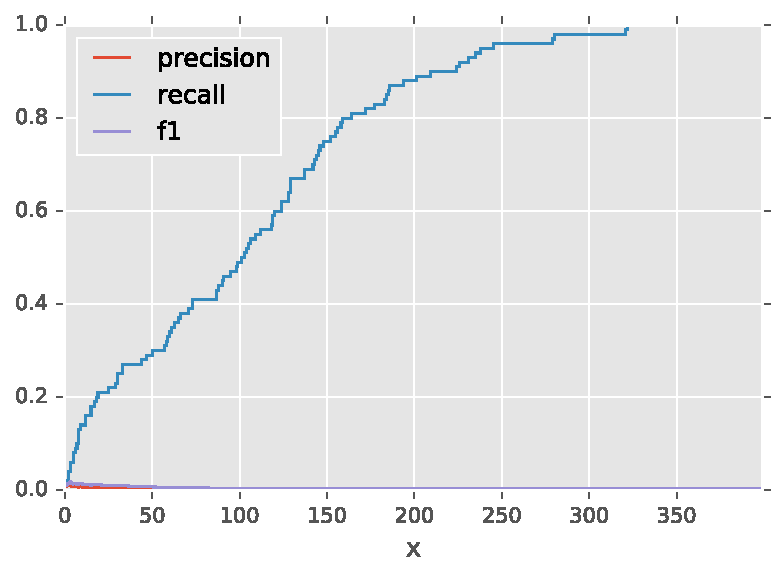
\includegraphics[]{figures/reddit-entertainment-f1.pdf}
\caption{``entertainment''}
\label{fig-reddit-entertainment-f1}
\end{subfigure}
\begin{subfigure}[t]{.4\textwidth}
\centering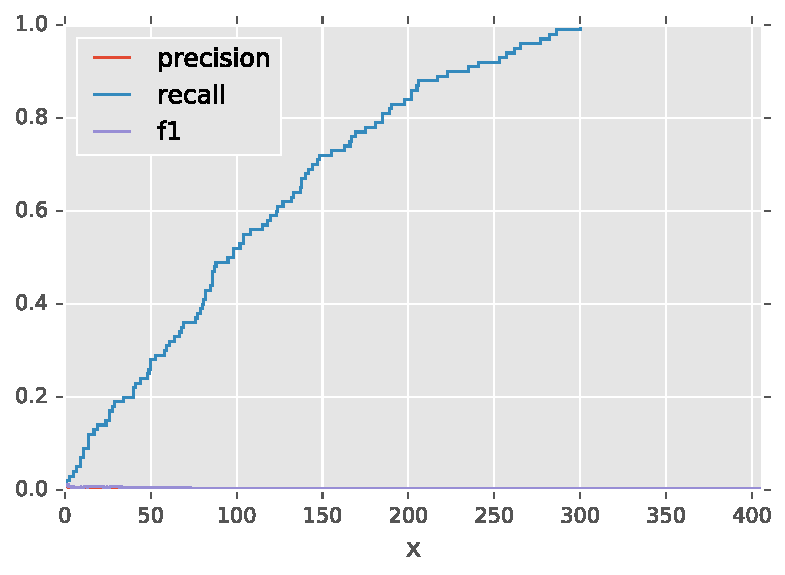
\includegraphics[]{figures/reddit-gaming-f1.pdf}
\caption{``gaming''}
\label{fig-reddit-gaming-f1}
\end{subfigure}
\begin{subfigure}[t]{.4\textwidth}
\centering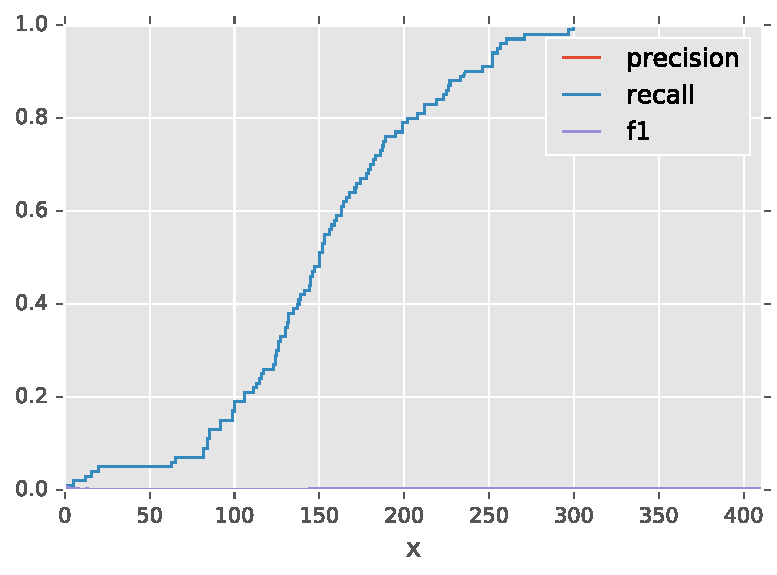
\includegraphics[]{figures/reddit-humor-f1.pdf}
\caption{``humor''}
\label{fig-reddit-humor-f1}
\end{subfigure}
\begin{subfigure}[t]{.4\textwidth}
\centering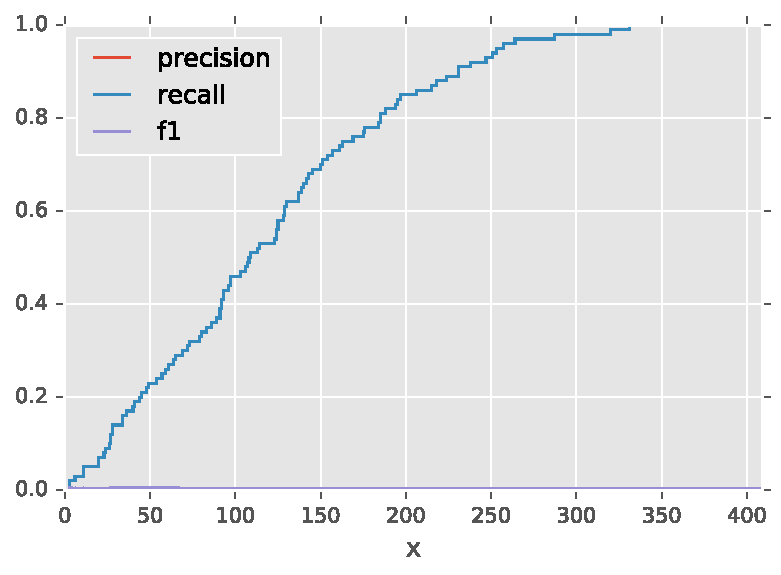
\includegraphics[]{figures/reddit-learning-f1.pdf}
\caption{``learning''}
\label{fig-reddit-learning-f1}
\end{subfigure}
\begin{subfigure}[t]{.4\textwidth}
\centering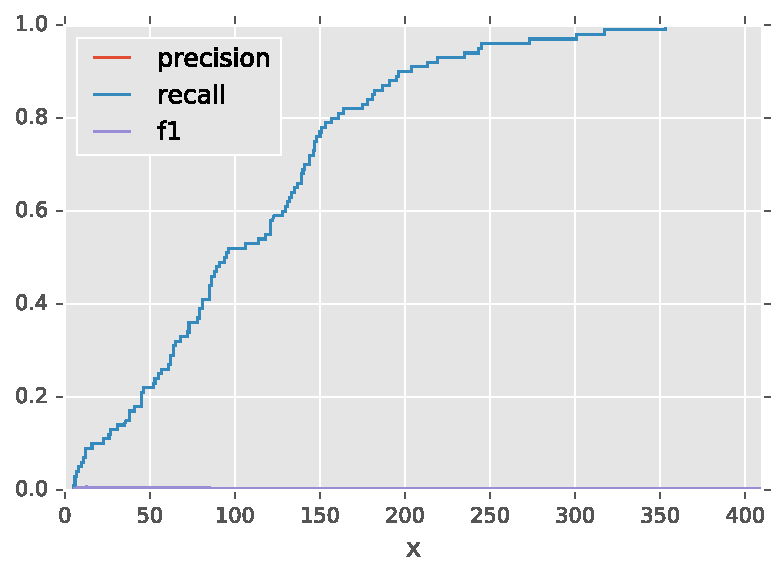
\includegraphics[]{figures/reddit-lifestyle-f1.pdf}
\caption{``lifestyle''}
\label{fig-reddit-lifestyle-f1}
\end{subfigure}
\begin{subfigure}[t]{.4\textwidth}
\centering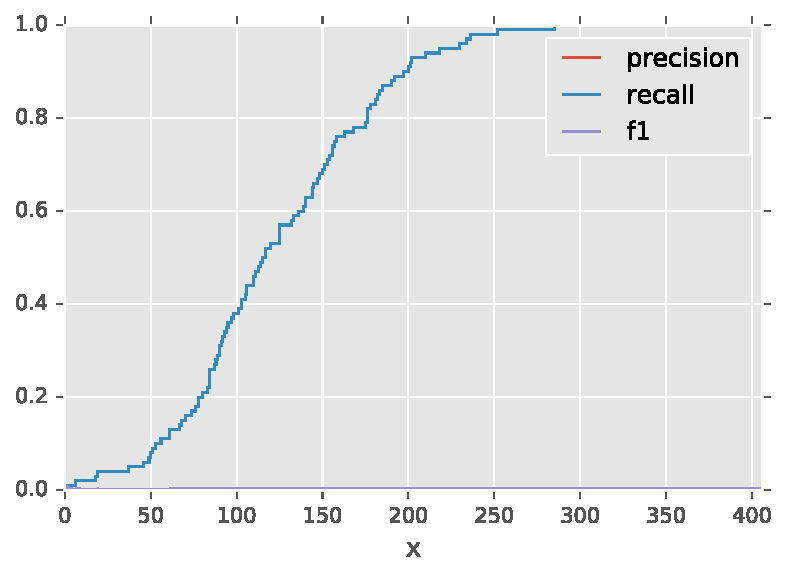
\includegraphics[]{figures/reddit-news-f1.pdf}
\caption{``news''}
\label{fig-reddit-news-f1}
\end{subfigure}
\begin{subfigure}[t]{.4\textwidth}
\centering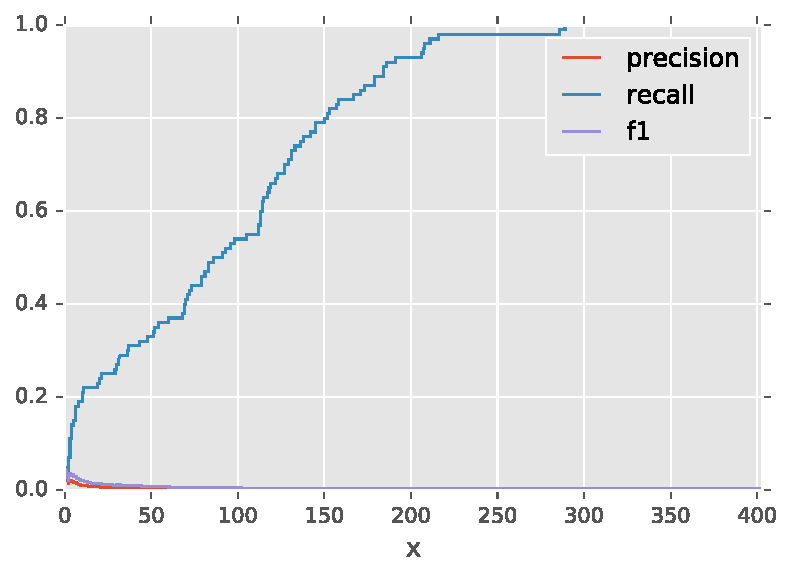
\includegraphics[]{figures/reddit-television-f1.pdf}
\caption{``television''}
\label{fig-reddit-television-f1}
\end{subfigure}
\caption{The precision, recall, and F1 score of codeword detection for $C_c$ being the hard synthetic Reddit corpus for each of the communities and $C_r$ being the original Reddit corpus.}
\label{fig-reddit-community-f1}
\end{figure}

\newpage

\subsubsection{Verifying the Community Effect}

To further verify that this is indeed the root cause (and not an idiosyncratic effect of the communities in and of themselves) I ran 7 more experiments. Each time, the codeword corpus is \textbf{the substituted subset of the original Reddit corpus belonging to the community} and the reference corpus is \textbf{the subset of the original Reddit corpus belonging to the community}. For example, for the ``humor'' experiment, I will substitute words only within the ``humor'' community, then run Word2Vec on only the ``humor'' community to produce the codeword embeddings. Then, I will take the original corpus from only the ``humor'' community, then run Word2Vec on the original ``humor'' community to produce reference embeddings. In other words, I am isolate each of the individual communities. If there was an idiosyncratic effect on a community level, this should produce bad results. However, if the bad results in the previous section were really the effect of codeword communities existing within a larger population, then the results for this section should be good.

As shown in Figures \ref{fig-reddit-community-only-count} and \ref{fig-reddit-community-only-f1}, the experiments consistently scored highly. The codewords were detected consistently. Hence, I conclude that it is the only the existence of communities that use a word within a codeword context existing within a population that uses the same word in the normal context that causes the problems in the previous experiment.

\begin{figure}[H]
\begin{subfigure}[t]{.4\textwidth}
\centering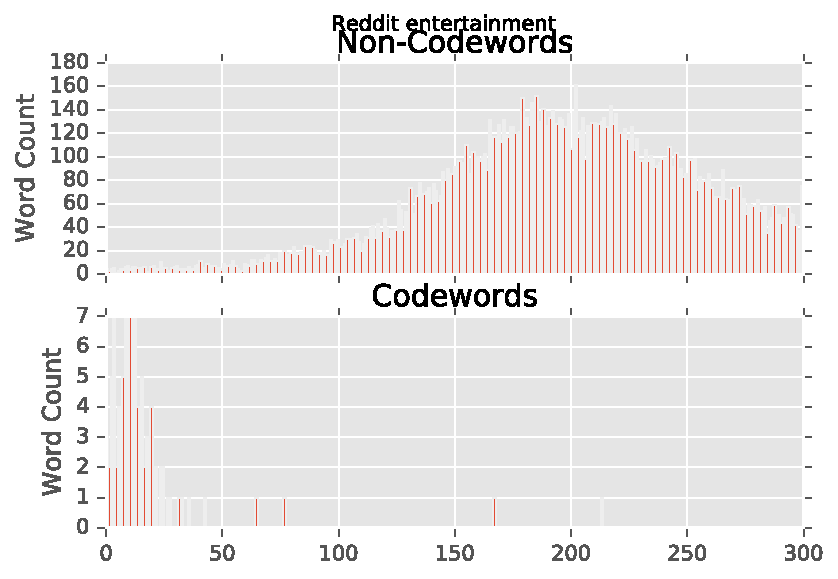
\includegraphics[]{figures/reddit-entertainment-only-count.pdf}
\caption{``entertainment'' only}
\label{fig-reddit-entertainment-only-count}
\end{subfigure}
\begin{subfigure}[t]{.4\textwidth}
\centering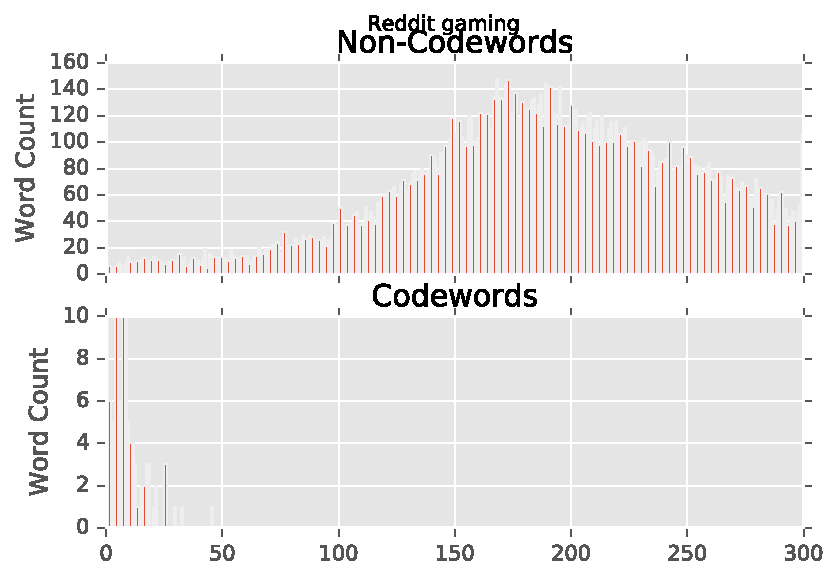
\includegraphics[]{figures/reddit-gaming-only-count.pdf}
\caption{``gaming'' only}
\label{fig-reddit-gaming-only-count}
\end{subfigure}
\begin{subfigure}[t]{.4\textwidth}
\centering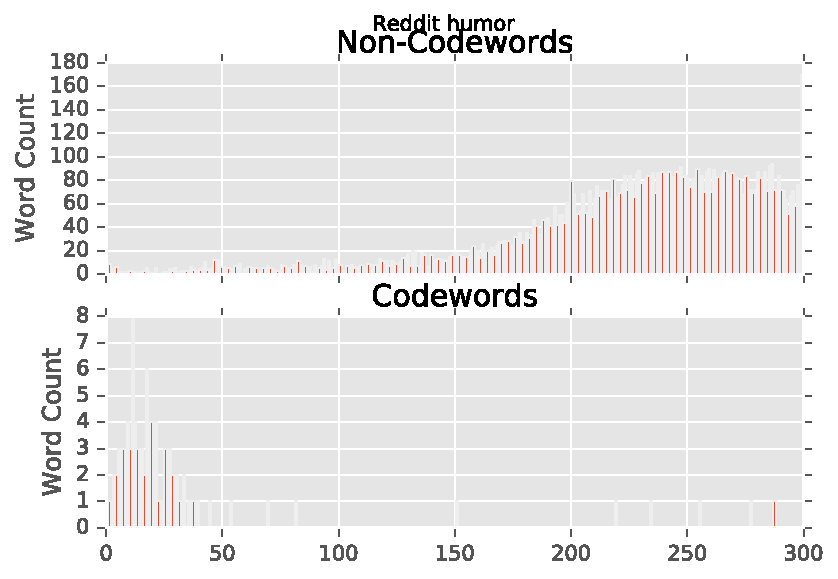
\includegraphics[]{figures/reddit-humor-only-count.pdf}
\caption{``humor'' only}
\label{fig-reddit-humor-only-count}
\end{subfigure}
\begin{subfigure}[t]{.4\textwidth}
\centering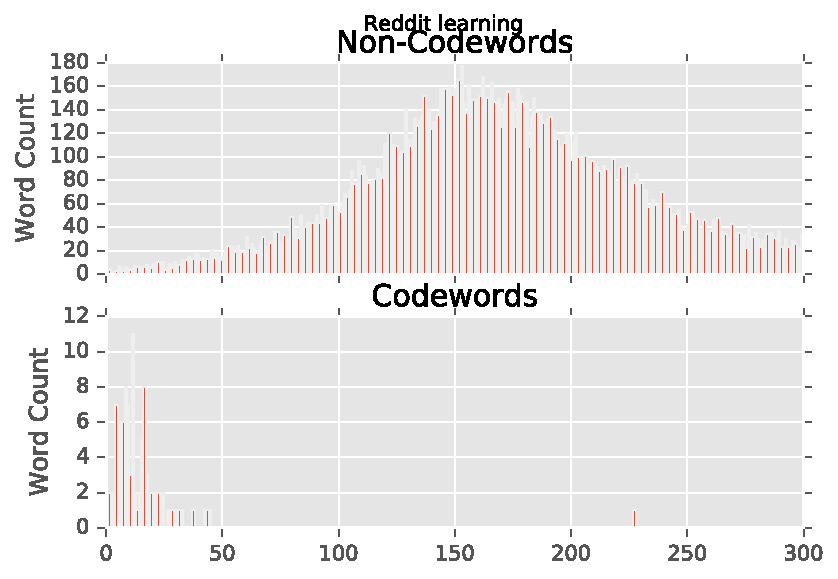
\includegraphics[]{figures/reddit-learning-only-count.pdf}
\caption{``learning'' only}
\label{fig-reddit-learning-only-count}
\end{subfigure}
\begin{subfigure}[t]{.4\textwidth}
\centering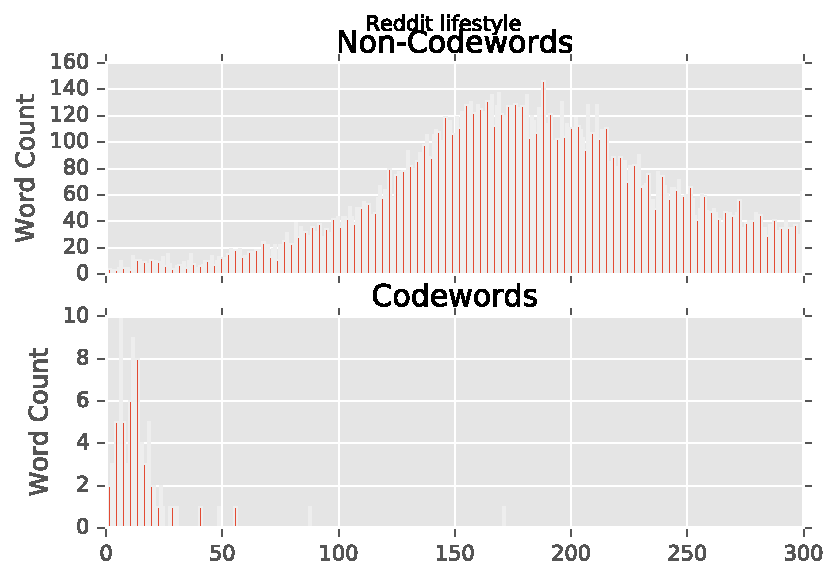
\includegraphics[]{figures/reddit-lifestyle-only-count.pdf}
\caption{``lifestyle'' only}
\label{fig-reddit-lifestyle-only-count}
\end{subfigure}
\begin{subfigure}[t]{.4\textwidth}
\centering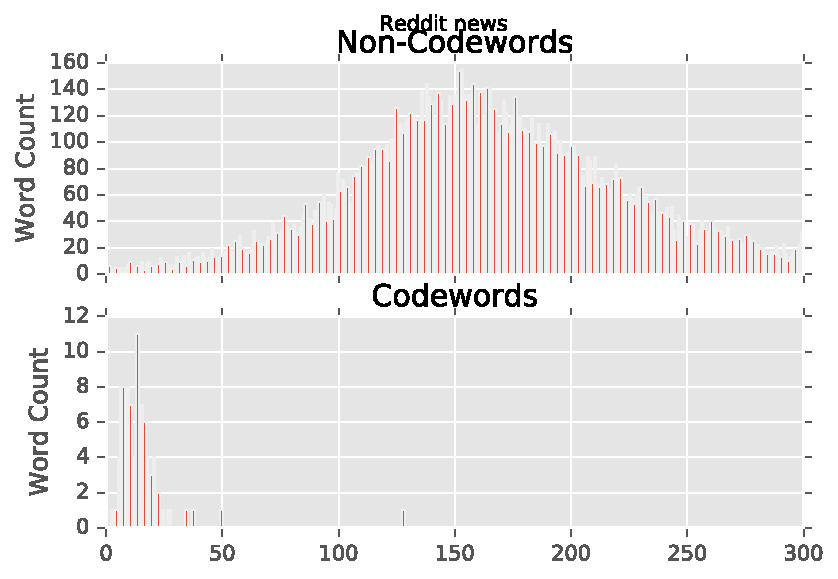
\includegraphics[]{figures/reddit-news-only-count.pdf}
\caption{``news'' only}
\label{fig-reddit-news-only-count}
\end{subfigure}
\begin{subfigure}[t]{.4\textwidth}
\centering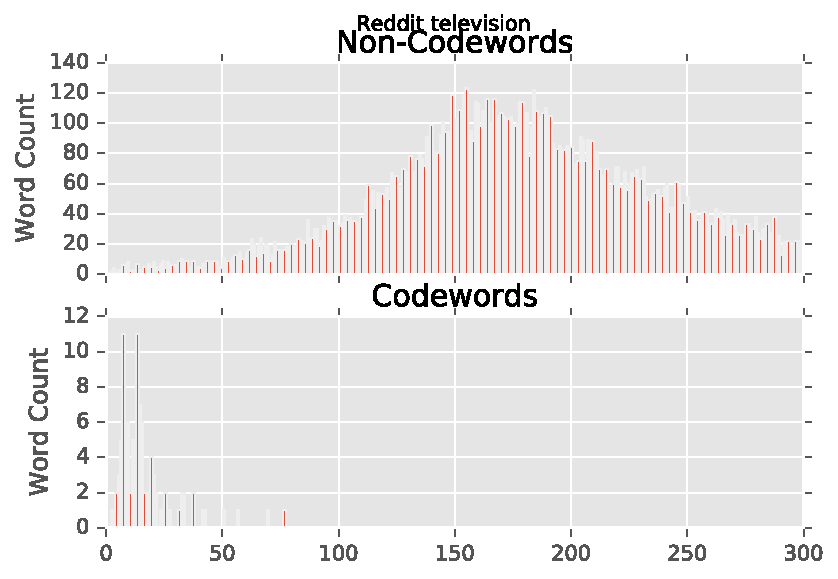
\includegraphics[]{figures/reddit-television-only-count.pdf}
\caption{``television'' only}
\label{fig-reddit-television-only-count}
\end{subfigure}
\caption{$x$ for non-codewords and codewords generated for every word $w_{i, c}$ and $w_{i, r}$, with $C_c$ being the subset of the synthetic Reddit corpus (codewords only the communities) and $C_r$ being the original Reddit corpus.}
\label{fig-reddit-community-only-count}
\end{figure}

\begin{figure}[H]
\begin{subfigure}[t]{.4\textwidth}
\centering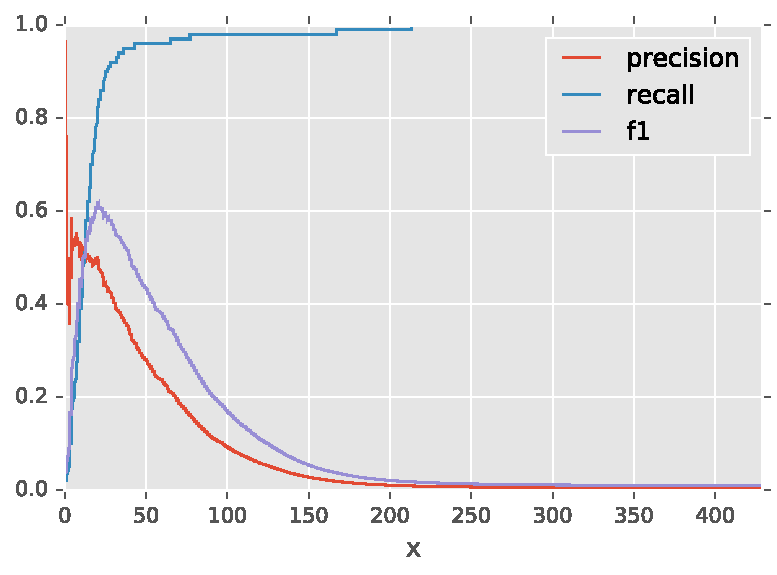
\includegraphics[]{figures/reddit-entertainment-only-f1.pdf}
\caption{``entertainment'' only}
\label{fig-reddit-entertainment-only-f1}
\end{subfigure}
\begin{subfigure}[t]{.4\textwidth}
\centering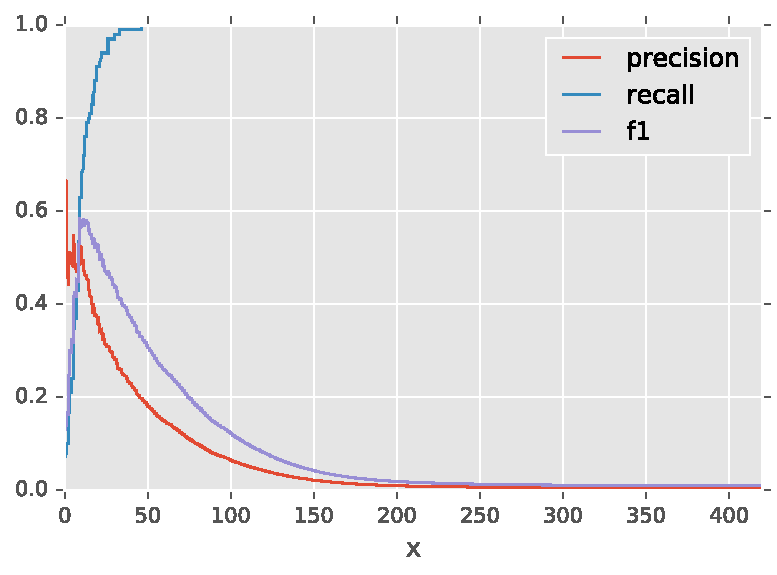
\includegraphics[]{figures/reddit-gaming-only-f1.pdf}
\caption{``gaming'' only}
\label{fig-reddit-gaming-only-f1}
\end{subfigure}
\begin{subfigure}[t]{.4\textwidth}
\centering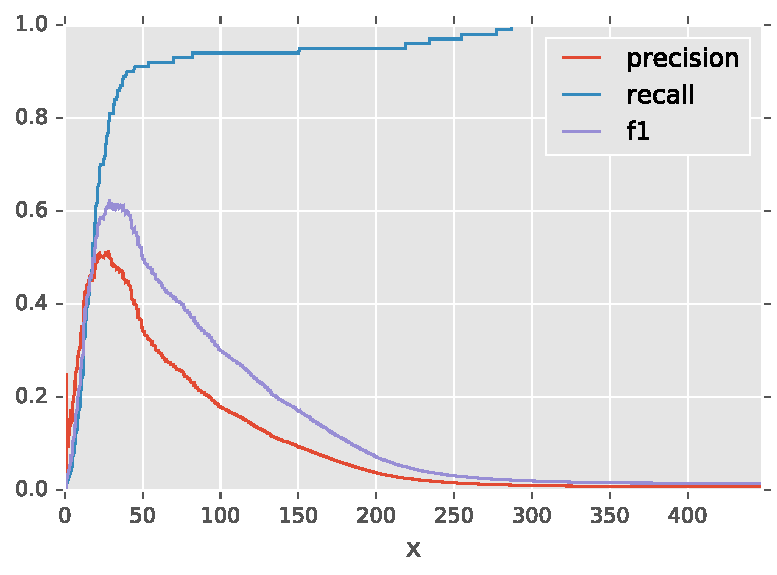
\includegraphics[]{figures/reddit-humor-only-f1.pdf}
\caption{``humor'' only}
\label{fig-reddit-humor-only-f1}
\end{subfigure}
\begin{subfigure}[t]{.4\textwidth}
\centering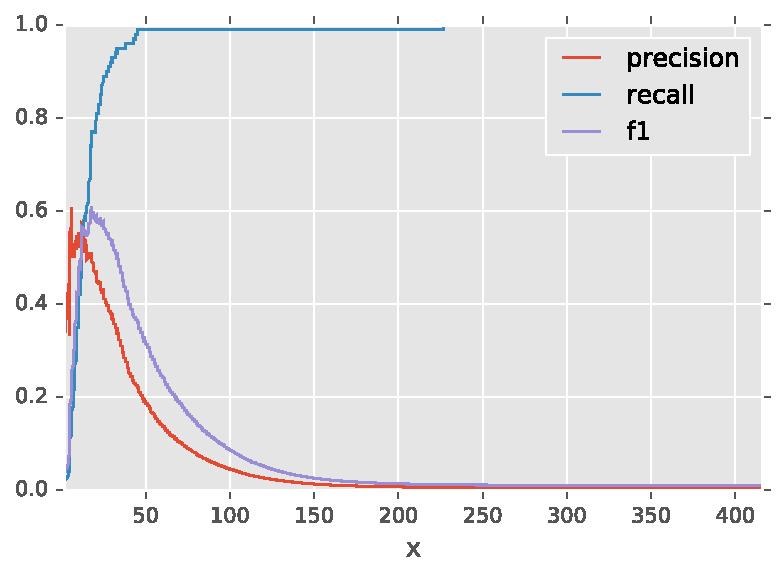
\includegraphics[]{figures/reddit-learning-only-f1.pdf}
\caption{``learning'' only}
\label{fig-reddit-learning-only-f1}
\end{subfigure}
\begin{subfigure}[t]{.4\textwidth}
\centering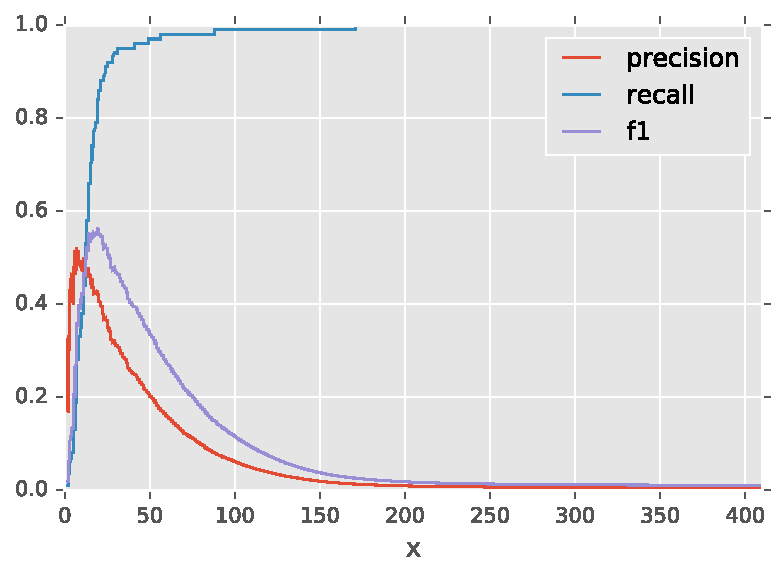
\includegraphics[]{figures/reddit-lifestyle-only-f1.pdf}
\caption{``lifestyle'' only}
\label{fig-reddit-lifestyle-only-f1}
\end{subfigure}
\begin{subfigure}[t]{.4\textwidth}
\centering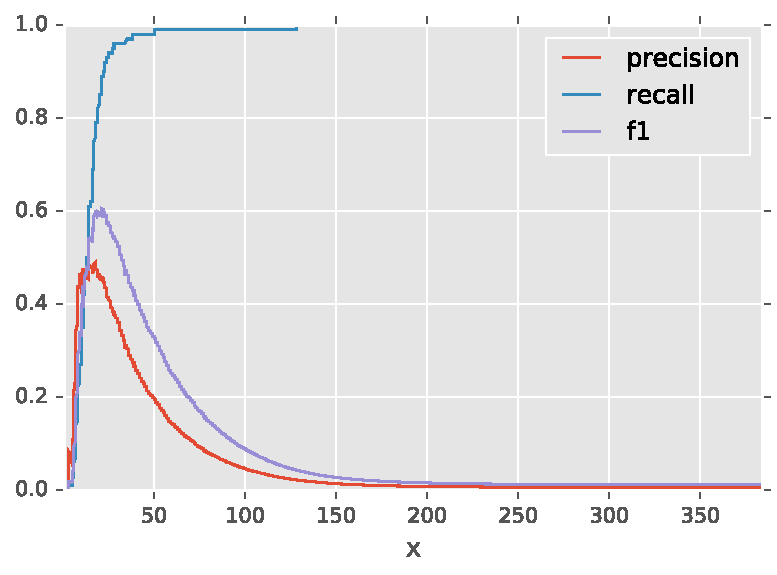
\includegraphics[]{figures/reddit-news-only-f1.pdf}
\caption{``news'' only}
\label{fig-reddit-news-only-f1}
\end{subfigure}
\begin{subfigure}[t]{.4\textwidth}
\centering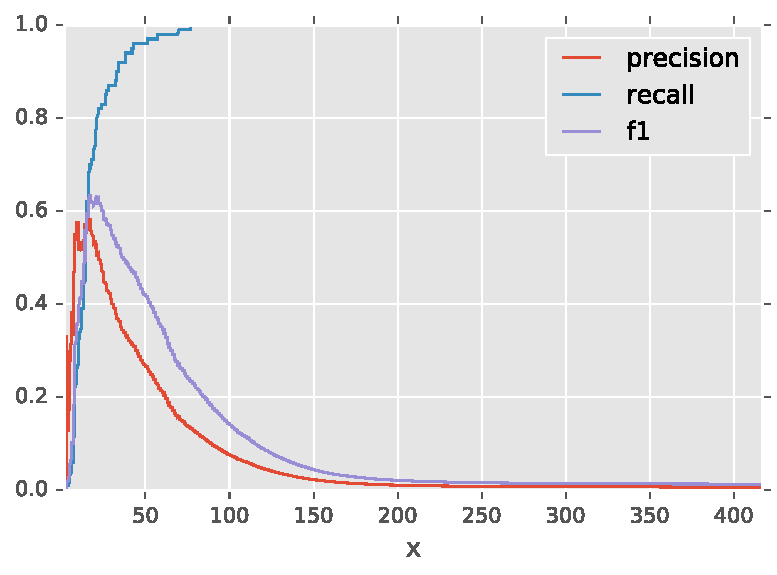
\includegraphics[]{figures/reddit-television-only-f1.pdf}
\caption{``television'' only}
\label{fig-reddit-television-only-f1}
\end{subfigure}
\caption{The precision, recall, and F1 score of codeword detection for $C_c$ being the subset of the synthetic Reddit corpus for each of the communities and $C_r$ being the original Reddit corpus.}
\label{fig-reddit-community-only-f1}
\end{figure}

\section{Polysemic Approach}

A deficiency in the prior approach is that each word has only one embedding. The \textbf{polysemy} (same word, different meanings / contexts) are ignored. In order to tackle polysemy, I need to find embedding methods that assign multiple embeddings to a single word. This is known as \textbf{Multi Sense Embeddings}, and Apoorv pointed me to \cite{neelakantan2015efficient} for a state of the art multi sense word embedding model.

Before I discuss that model, it is useful to review the Skip-gram with negative sampling model used by Word2Vec since the multi sense embedding model is an extension of the original skipgram model.

\subsection{Background on Skip-gram with Negative Sampling}

The Skip-gram model assumes that words have contexts based on the words around them, and do not have contexts with words that are far away from them. This is known as the distributional hypothesis. In the skipgram model, $v(w_{i, x}) \in R^d$ is the vector representation of the word $w_{i, x}$ for $i \in 1 ... n$ where $n$ is the number of words in the corpus, and $C_x$ is the corpus. $d$ is the dimensionality of the embedding. Given a pair of words $(w_{i, x}, c)$, the probability that the word $c$ (for context) is observed in the context of word $w_{i, x}$ is given by

\[ P(D = 1 | v(w_{i, x}), v(c)) = \frac{1}{1+\exp{-v(w_{i, x})^n v(c)}}\]

The probability of not observing the word $c$ in the context of $w_{i, x}$ is given by

\[ P(D = 0 | v(w_{i, x}), v(c)) = 1 - P(D = 1 | v(w_{i, x}), v(c)) = 1 - \frac{1}{1+\exp{-v(w_{i, x})^n v(c)}}\]

Give na training set containing the sequence of words $w_{1, x}, w_{2,x} ... w_{n, x}$, the word embeddings are learned by maximizing the objective function:

\begin{align*}
J(\theta) = &\sum_{(w_{i, x}, c_{i, x}) \in G^+} \sum_{c \in c_{i, x}} \log{P(D=1 | v(w_{i,x}), v(c)})\\
&+ \sum_{(w_{i, x}, c_{i, x}) \in G^-} \sum_{c' \in c'_{i, x}} \log{P(D=0 | v(w_{i,x}), v(c')})
\end{align*}

where $w_{i, x}$ is the $i$th word in the training corpus $C_x$, $c_{i, x}$ is the set of observed context words of word $w_{i, x}$ and $c'_{i, x}$ is the set of randomly selected noisy context words for the word $w_{i, x}$. $G^+$ consists of the set of all observed word-context pairs $(w_{i, x}, c_{i, x})$ where $i \in 1 ... n$. $G^-$ consists of the pairs $(w_{i,x}, c'_{i, x})$ where $i \in 1 ... n$ where $c'_{i, x}$ is the set of randomly selected noisy context words for the word $w_{i, x}$.

For each training word $w_{i, x}$ the set of context words $c_{i, x} = \{ w_{i - R_i, x} ... w_{i - 1, x} w_{i + 1, x} ... w_{i + R_i, x} \}$ which includes $R_i$ words to the left and right of the given word. $R_i$ is the window size considered for the word $w_{i,x}$ uniformly randomly sampled from the set $1 ... W$ where $W$ is the maximum context window size.

The set of noisy context words $c'_{i, x}$ is constructed by randomly sampling $S$ noisy context words for each word in the context $c_{i, x}$. The noisy context words are randomly sampled from the following distribution:

\[P(w_{i, x}) = \frac{P_{unigram}(w_{i,x})^\frac{3}{4}}{Z}\]

where $P_{unigram}(w_{i,x})$ is the unigram distribution of the words and $Z$ is the normalization constant.

\subsection{Multi Sense Skipgram Model}

\cite{neelakantan2015efficient} extended the skip-gram model by letting each \textbf{sense} of word have its own embedding.

\begin{quote}
(We) let each sense of word have its own embed- ding, and induce the senses by clustering the em- beddings of the context words around each token. The vector representation of the context is the average of its context words’ vectors. For every word type, we maintain clusters of its contexts and the sense of a word token is predicted as the cluster that is closest to its context representation. After predicting the sense of a word token, we perform a gradient update on the embedding of that sense. The crucial difference from previous approaches is that word sense discrimination and learning em- beddings are performed jointly by predicting the sense of the word using the current parameter estimates.\footnote{\cite{neelakantan2015efficient}}
\end{quote}

In the extended model, each word $w_{i,x}$ is associated with a global vector $v_g(w_{i,x})$ and each sense of the word has an embedding $v_s(w_{i,x}, k)$ for $k \in 1 ... K$ where $K$ is the number of senses of the word. Each sense of the word is also associated with a context cluster with center $\mu(w_{i,x}, k)$ for $k \in 1 ... K$. $K$ and the dimension of the vectors $d$ are hyperparameters.

Let's say I have a word $w_{i,x}$. The context of that word is $c_{i, x} = \{w_{i-R_i, x} ... w_{i-1, x} w_{i+1, x} ... w_{i+R_i,x}\}$ based on the observed context words. The vector representation of the context is defined as the average of the global vector representation of the words in the context. Hence,

\[v_{context}(c_{i,x}) = \frac{1}{2R_i}\sum_{c \in c_{i, x}} v_g(c)\]

\cite{neelakantan2015efficient} used the global vectors of the context words instead of the sense vectors to avoid the computational complexity associated with predicting the sense of the context words. Then, the algorithm predicts $s_{i, x}$, the sense of the word $w_{i,x}$ when associated with the context $c_{i, x}$ using the existing cluster centers of the sense vectors of the word $w_{i,x}$. This portion of the algorithm is similar to the k-means algorithm. The chosen sense $s_{i,x}$ is essentially

\[s_{i,x} = \mathrm{argmax}_{k \in 1 ... K} cossim(\mu(w_{i,x}, k), v_{context}(c_{i,x}))\]

The cluster center is the average of the vector representation of all the contexts which belong to that cluster. $cossim$ is simply the cosine similarity measure used in earlier experiments.

The probability that word $c$ is observed in the context of word $w_{i, x}$ given the sense of word $w_{i,x}$ is

\begin{align*}
&P(D = 1 | s_{i,x}, v_s(w_{i,x}, 1), ... v_s(w_{i,x}, K), v_g(c)) \\
&= P(D=1|v_s(w_{i,x}, s_{i,x}), v_g(c)) \\
&= \frac{1}{1 + e^{-v_s(w_{i,x}, s_{i,x})^n v_g(c)}}
\end{align*}

The probability of not observin the word $c$ in the context of $w_{i,x}$ given the sense of word $w_{i,x}$ is:

\begin{align*}
&P(D = 0 | s_{i,x}, v_s(w_{i,x}, 1), ... v_s(w_{i,x}, K), v_g(c)) \\
&= P(D=0|v_s(w_{i,x}, s_{i,x}), v_g(c)) \\
&= 1 - P(D=1|v_s(w_{i,x}, s_{i,x}), v_g(c)) \\
&= \frac{1}{1 + e^{-v_s(w_{i,x}, s_{i,x})^n v_g(c)}}
\end{align*}

Given a training set containing the sequence of words $w_{1,x}, w_{2,x} ... w_{n,x}$ the word embeddings are learned by maximizing the objective function:

\begin{align*}
J(\theta) = &\sum_{(w_{i,x}, c_{i,x}) \in G^+} \sum_{c \in c_{i,x}} \log P(D = 1 | v_s(w_{i,x}, s_{i,x}), v_g(c)) \\
&+ \sum_{(w_{i,x}, c_{i,x}) \in G^-} \sum_{c' \in c'_{i,x}} \log P(D = 0 | v_s(w_{i,x}, s_{i,x}), v_g(c'))
\end{align*}

The variables $c$ $c'$ $G^+$ and $G^-$ are constructed in the same way as the original Skip-gram with negative sampling model. After predicting the sense of the word, the algorithm updates the embedding of the predicted sense of the word $w_{i,x}(v_s(w_{i,x}, s_{i,x}))$, the global vector of the words in the context and the global vector of the randomly sampled noisy context words. The context cluster center of cluster $s_{i,x}$ for the word $w_{i,x}$, $\mu(w_{i,x}, s_{i,x})$ is updated since context $c_{i,x}$ is updated to the cluster $s_{i,x}$.

By giving each word multiple senses, it disambiguates between different usages of the same word, a limitation that \texttt{word2vec} has as shown in Figure \ref{fig-mssg-demo}.

\begin{figure}[H]
\begin{itemize}
\item Skip-gram: 
\subitem blackberry, macintosh, acorn, pear, plum
\item MSSG:
\subitem pear, honey, pumpkin, potato, nut 
\subitem microsoft, activision, sony, retail, gamestop
\subitem macintosh, pc, ibm, iigs, chipsets
\end{itemize}
\caption{Words similar to the word ``apple''. Each sublist represents a different sense of the word ``apple''. For the original skip-gram model, only one sense is available. However, using the Multi-Sense Skipgram (MSSG) model, I am able to disambiguate between different senses of the word ``apple''}
\label{fig-mssg-demo}
\end{figure}

This is useful in the codeword detection problem. However, before tackling that, I wanted to ensure that the code runs first. A good trial run would be to test this code (which \cite{neelakantan2015efficient} provides at \url{https://bitbucket.org/jeevan_shankar/multi-sense-skipgram/overview} on the Reddit corpus to detect multiple senses of words.

Trying to compile this project using the given \texttt{make\_cp.sh} produces the following errors:

\begin{lstlisting}
(default)➜  multi-sense-skipgram git:(master) sh make_cp.sh
error: error while loading CharSequence, class file '/Library/Java/JavaVirtualMachines/jdk1.8.0_31.jdk/Contents/Home/jre/lib/rt.jar(java/lang/CharSequence.class)' is broken
(class java.lang.RuntimeException/bad constant pool tag 18 at byte 10)
error: error while loading Comparator, class file '/Library/Java/JavaVirtualMachines/jdk1.8.0_31.jdk/Contents/Home/jre/lib/rt.jar(java/util/Comparator.class)' is broken
(class java.lang.RuntimeException/bad constant pool tag 18 at byte 20)
error: error while loading AnnotatedElement, class file '/Library/Java/JavaVirtualMachines/jdk1.8.0_31.jdk/Contents/Home/jre/lib/rt.jar(java/lang/reflect/AnnotatedElement.class)' is broken
(class java.lang.RuntimeException/bad constant pool tag 18 at byte 76)
error: error while loading Arrays, class file '/Library/Java/JavaVirtualMachines/jdk1.8.0_31.jdk/Contents/Home/jre/lib/rt.jar(java/util/Arrays.class)' is broken
(class java.lang.RuntimeException/bad constant pool tag 18 at byte 765)
/var/folders/sw/0j_h3wdj6zjcpkyty1gw_rj00000gq/T/sbt_994f79e2/API.scala:424: error: java.util.Comparator does not take type parameters
	private[this] val sortClasses = new Comparator[Symbol] {
                                            ^
5 errors found
\end{lstlisting}

Turns out this can be resolved by uncommenting the line \lstinline{<useManifestOnlyJar>false</useManifestOnlyJar} in \texttt{pom.xml} for the code. Running the demo bash script would run NP-MSSG on the \texttt{text8} corpus.

\subsection{Modifying the MSSG Algorithm to Solve Community Problem}

In the codeword detection problem, we are interested in finding how different communities use the same words. For example, if ``cheeseburger'' was used by one single community to denote financial fraud while the rest of the communities use it to denote the food, the MSSG algorithm will tell us that there are two senses of the word ``cheeseburger''. However, to use this directly to solve this problem, I needed to modify the MSSG algorithm to tell me \textbf{how different communities utilize the different senses of the words}.

The key to the word sense association is $s_{i,x} = \mathrm{argmax}_{k \in 1 ... K} cossim(\mu(w_{i,x}, k), v_{context}(c_{i,x}))$ In other words, the sense chosen for a word encountered is the closest cluster center for the word's current average context (a word is associated with multiple cluster centers) in a process very similar to the k-means algorithm.

This process can be exploited to identify the community to which a word sense belongs. For example, let's say that there are 5 communities. Let's also say that ``apple'' has two word senses -- that of the fruit (so it will be associated with words like ``orange'' and ``banana'') and that of the company (so it will be associated with words like ``samsung'' and ``microsoft'').

Let's say that each word sense has an array of frequency counts attached to it that counts the number of times it is chosen as the cluster center in the step $s_{i,x} = \mathrm{argmax}_{k\in 1 ... K} \{sim(\mu(w_{i,x}, k), v_{context}(c_{i,x}))\}$. That means, if in the sentence ``Apple beats Samsung in latest sales.'', ``apple'' is associated the second cluster center, and this sentence appeared in the first community then $count_{\mu(apple, s_{i,x} = 2, community = 1)} += 1$. If in the sentence ``Apple and banana makes a good smoothie.'' is associated with the first cluster center and the sentence comes from the 5th community, then $count_{\mu(apple, s_{i,x} = 1, community = 5)} += 1$.

Then, at the end of training, we should have a histogram, for each word and for each word sense, of the frequency the word is attributed to each community. For example, I may have:

\begin{itemize}
\item For the first sense of the word apple ($s_{i,x} = 1$) in the sense of fruit
\begin{itemize}
\item $count_{\mu(apple, s_{i,x}=1, community=1)} = 5069$
\item $count_{\mu(apple, s_{i,x}=1, community=2)} = 4839$
\item $count_{\mu(apple, s_{i,x}=1, community=3)} = 5143$
\item $count_{\mu(apple, s_{i,x}=1, community=4)} = 3948$
\item $count_{\mu(apple, s_{i,x}=1, community=5)} = 4510$
\end{itemize}
\item For the first sense of the word apple ($s_{i,x} = 2$) in the sense of the company
\begin{itemize}
\item $count_{\mu(apple, s_{i,x}=2, community=1)} = 534$
\item $count_{\mu(apple, s_{i,x}=2, community=2)} = 134$
\item $count_{\mu(apple, s_{i,x}=2, community=3)} = 314$
\item $count_{\mu(apple, s_{i,x}=2, community=4)} = 134$
\item $count_{\mu(apple, s_{i,x}=2, community=5)} = 24506$
\end{itemize}
\end{itemize}

What I may see is that the first sense of the word is pretty evenly distributed across the communities. This means that all the communities are using the word apple in the first sense. However, for the apple company word sense, only the 5th community is using it significantly. This implies that apple as a company is unique in meaning to the 5th community.

This is then directly relevant to codeword detection. A codeword is by definition \textbf{a word that a specific subset of people in an organization (a community) uses differently from others}. Let's say that I were able to identify these communities via a separate method (probably social clustering). Then, given these communities, I would now be able to identify \emph{lingo} that is specific to a community (a subset of the entire organization). Let's say that traders in department x is using the word ``cheeseburger'' to denote an offshore account. Then, the sense of the word ``cheeseburger'' as an offshore account would have high counts for that specific community.

I do note that not only codewords may be detected -- certain communities may simply use words that are unique to their community (e.g. slangs). Nonetheless, these will be interesting in the legal discovery process as well and would be interesting to be identified.

This requires a modification to the NP-MSSG that has a special data structure to label each word with its provenance. This was done in Scala. The output is, along with the original embeddings, a histogram of community counts for each sense of a word $w_{i,x}$.

\begin{landscape}

\begin{figure}[H]
\begin{subfigure}[t]{.3\textwidth}
\centering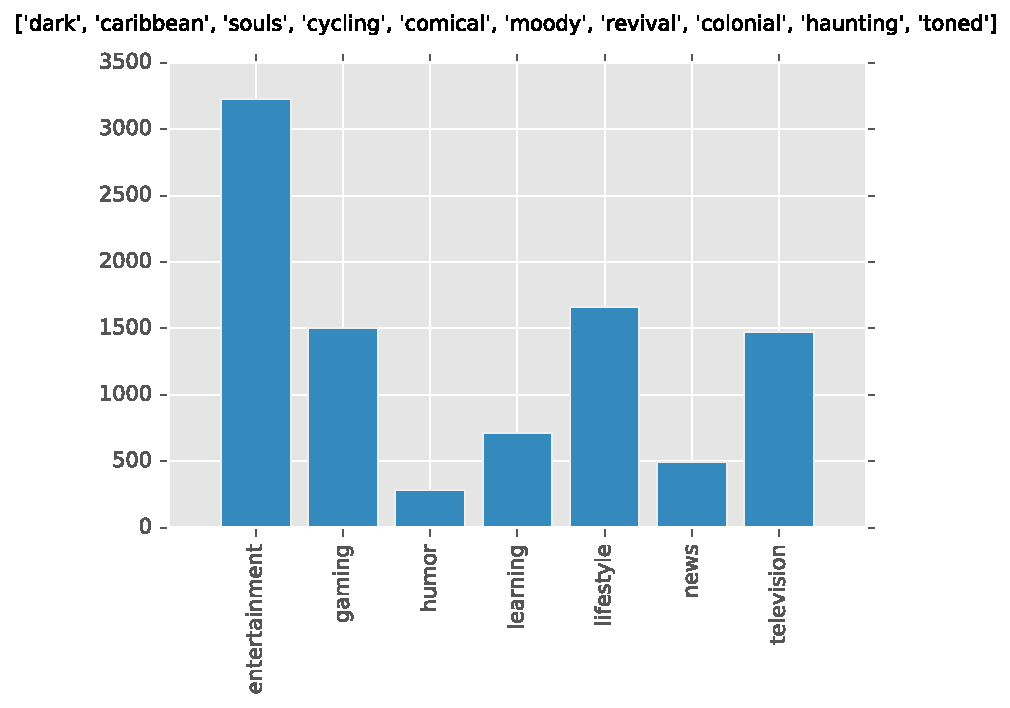
\includegraphics[]{figures/reddit-dark-0.pdf}
\caption{``dark'' sense 1}
\label{fig-reddit-dark-0}
\end{subfigure}
\begin{subfigure}[t]{.3\textwidth}
\centering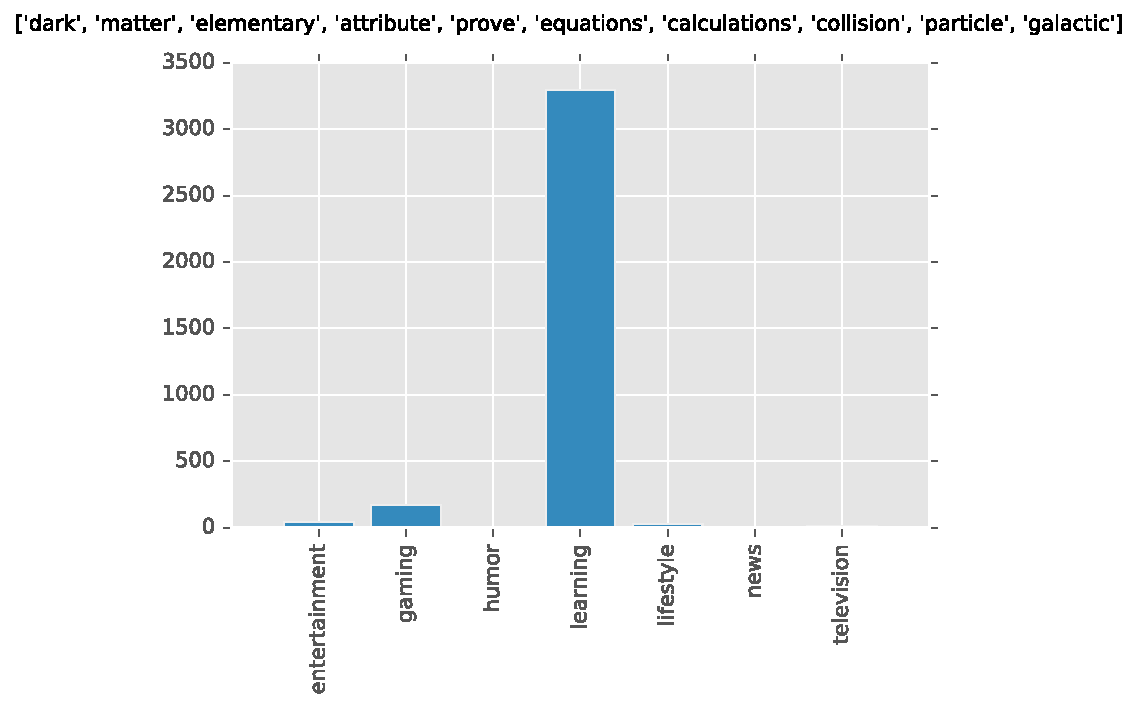
\includegraphics[]{figures/reddit-dark-1.pdf}
\caption{``dark'' sense 2}
\label{fig-reddit-dark-1}
\end{subfigure}
\begin{subfigure}[t]{.3\textwidth}
\centering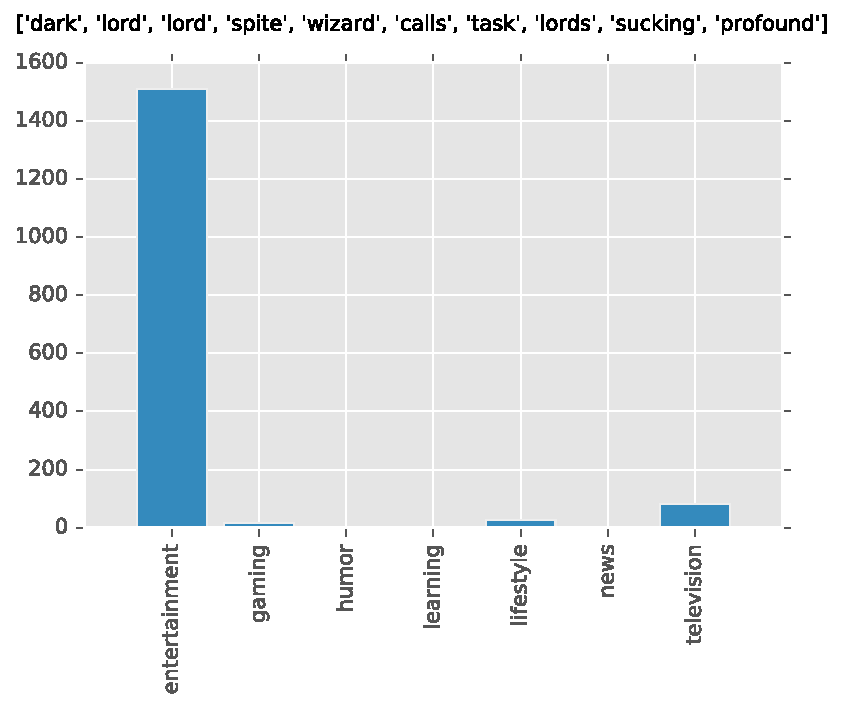
\includegraphics[]{figures/reddit-dark-2.pdf}
\caption{``dark'' sense 3}
\label{fig-reddit-dark-2}
\end{subfigure}
\begin{subfigure}[t]{.3\textwidth}
\centering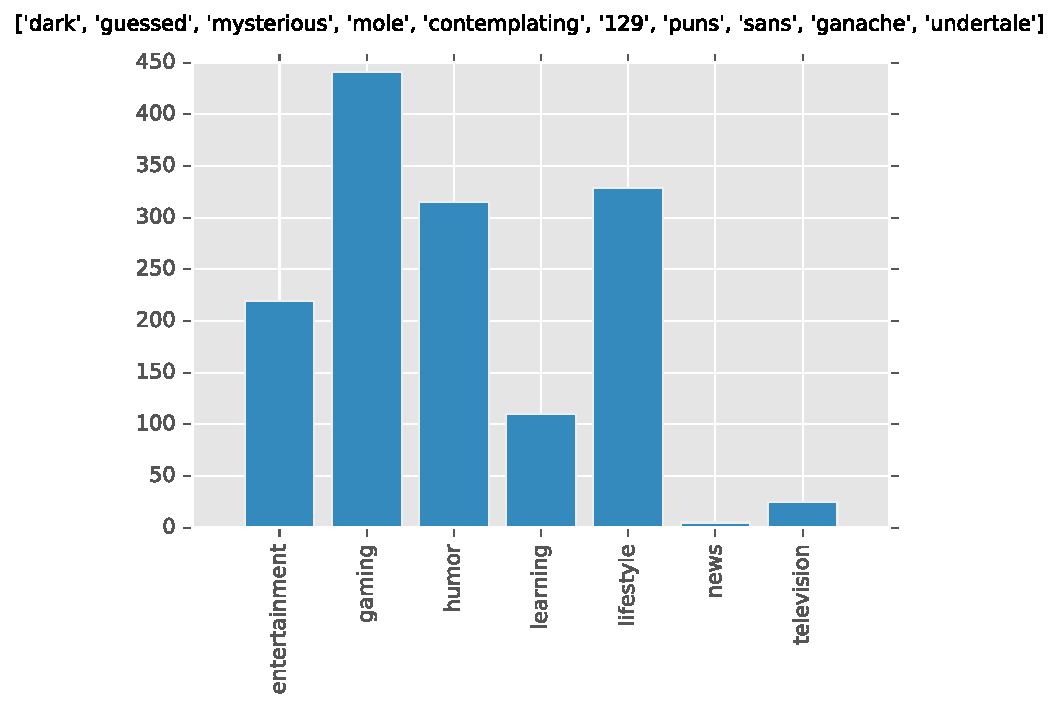
\includegraphics[]{figures/reddit-dark-3.pdf}
\caption{``dark'' sense 4}
\label{fig-reddit-dark-3}
\end{subfigure}
\begin{subfigure}[t]{.3\textwidth}
\centering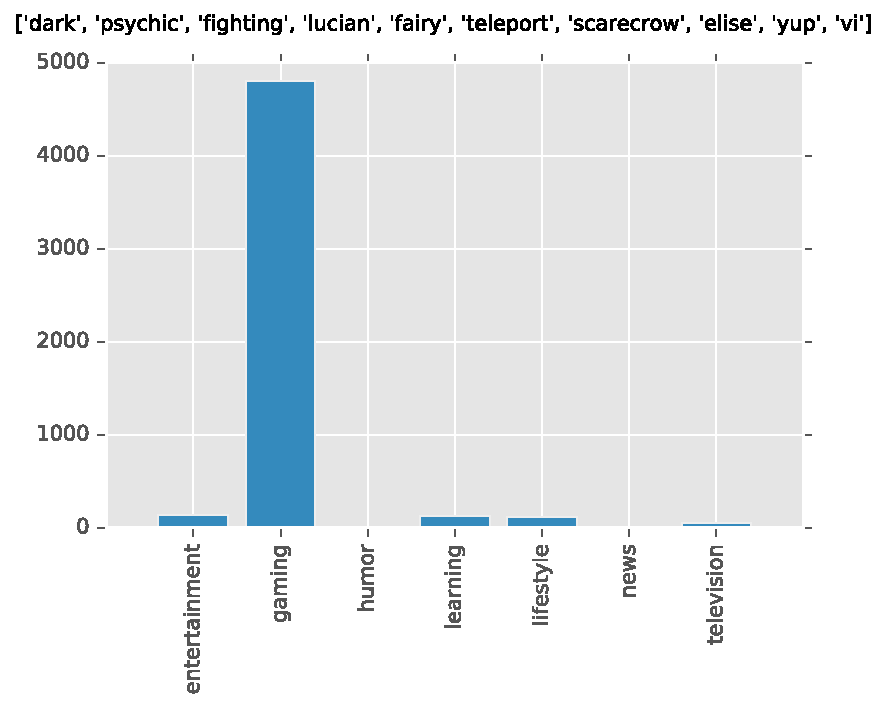
\includegraphics[]{figures/reddit-dark-4.pdf}
\caption{``dark'' sense 5}
\label{fig-reddit-dark-4}
\end{subfigure}
\begin{subfigure}[t]{.3\textwidth}
\centering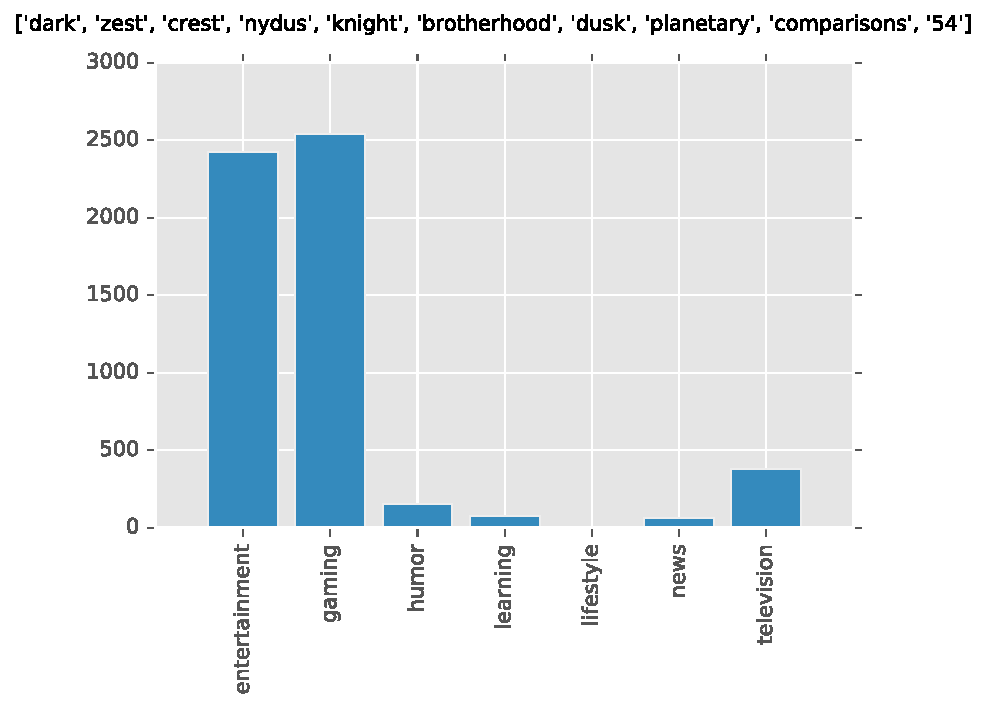
\includegraphics[]{figures/reddit-dark-5.pdf}
\caption{``dark'' sense 6}
\label{fig-reddit-dark-5}
\end{subfigure}
\begin{subfigure}[t]{.3\textwidth}
\centering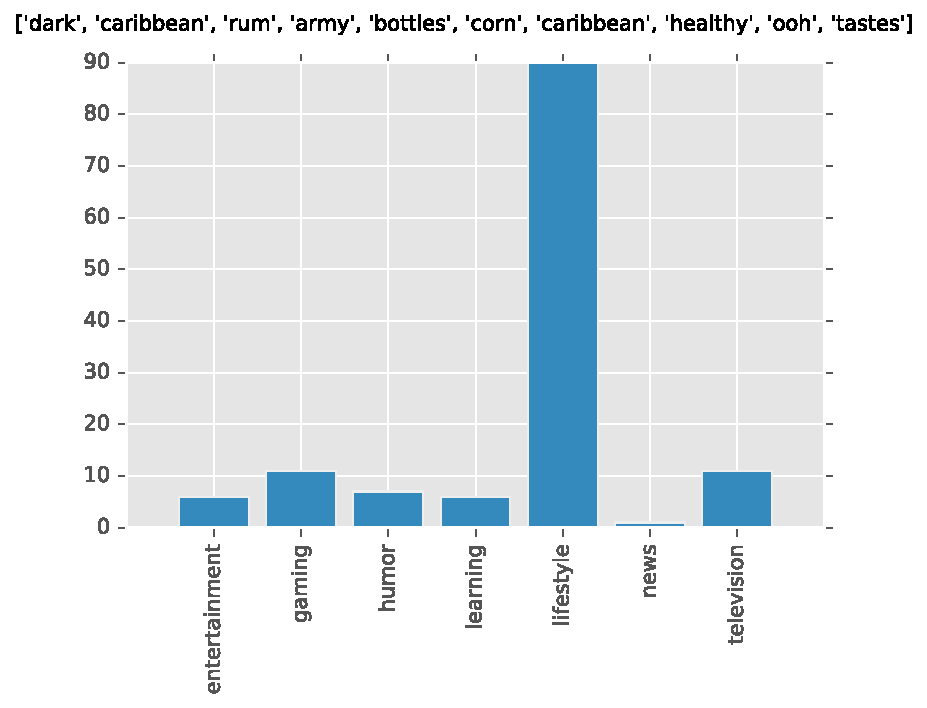
\includegraphics[]{figures/reddit-dark-6.pdf}
\caption{``dark'' sense 1}
\label{fig-reddit-dark-7}
\end{subfigure}
\caption{The different senses of the word ``dark'' together with the words most similar to the particular sense of ``dark''.}
\label{fig-reddit-dark} 
\end{figure}

\begin{figure}[H]
\begin{subfigure}[t]{.3\textwidth}
\centering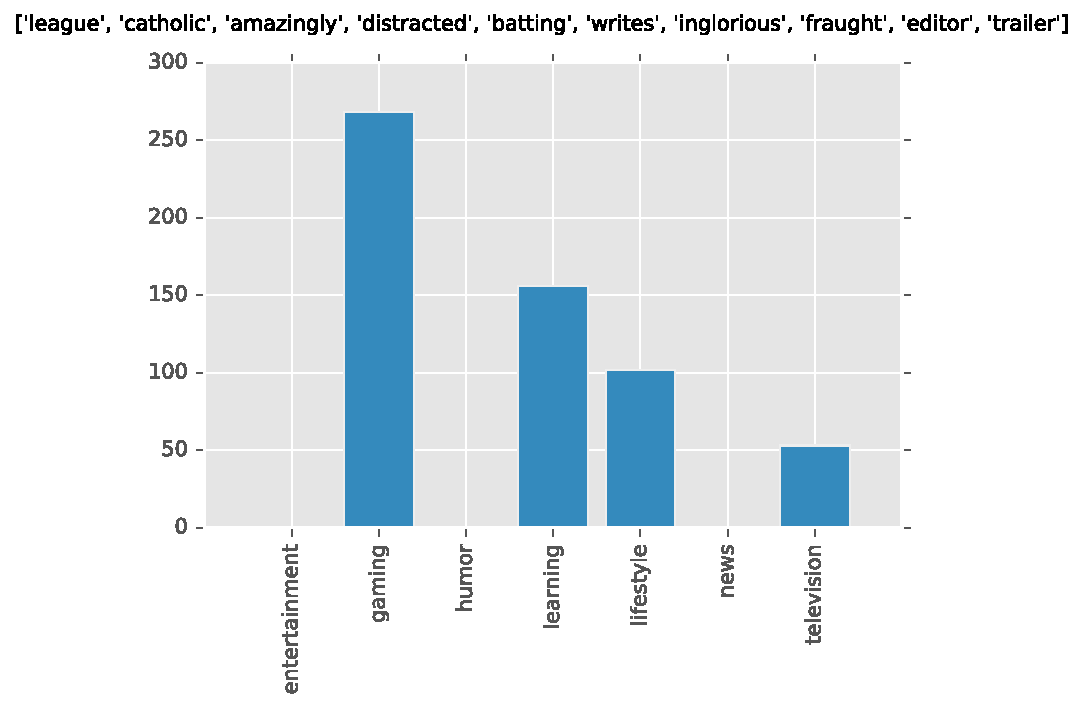
\includegraphics[]{figures/reddit-league-0.pdf}
\caption{``league'' sense 1}
\label{fig-reddit-league-0}
\end{subfigure}
\begin{subfigure}[t]{.3\textwidth}
\centering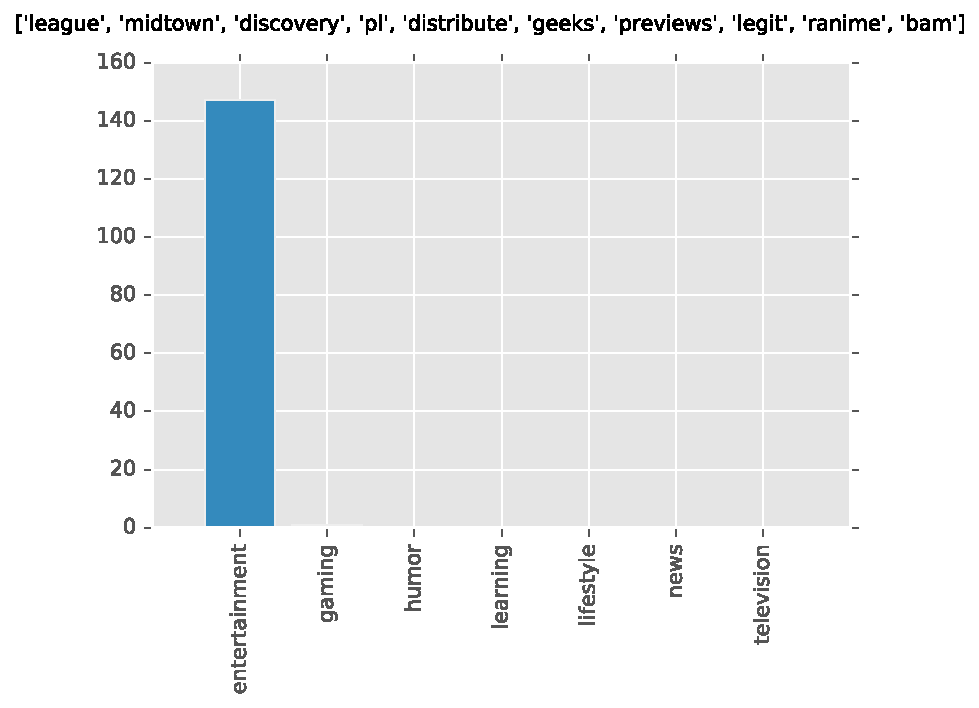
\includegraphics[]{figures/reddit-league-1.pdf}
\caption{``league'' sense 2}
\label{fig-reddit-league-1}
\end{subfigure}
\begin{subfigure}[t]{.3\textwidth}
\centering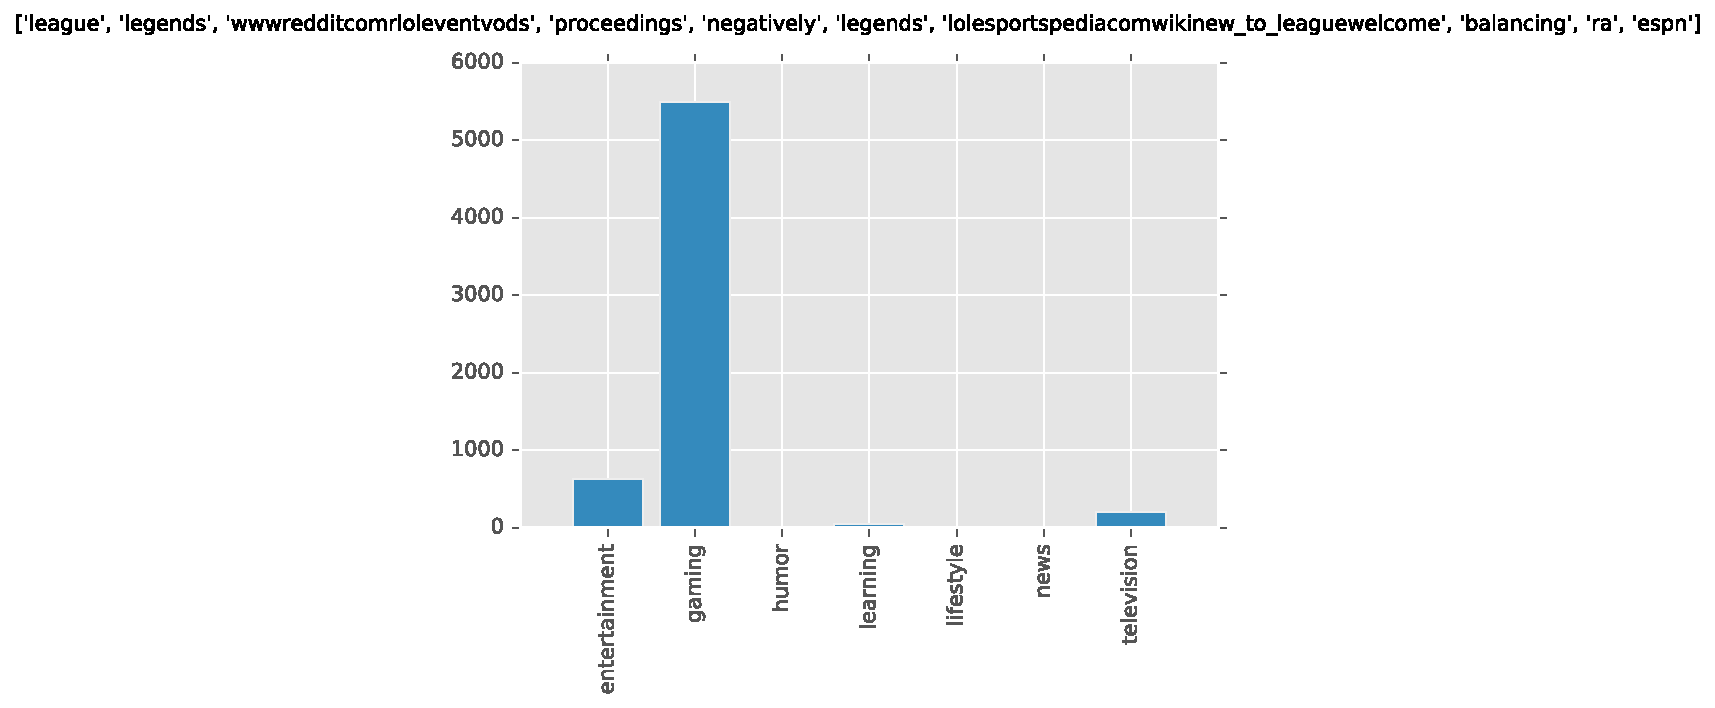
\includegraphics[]{figures/reddit-league-2.pdf}
\caption{``league'' sense 3}
\label{fig-reddit-league-2}
\end{subfigure}
\begin{subfigure}[t]{.3\textwidth}
\centering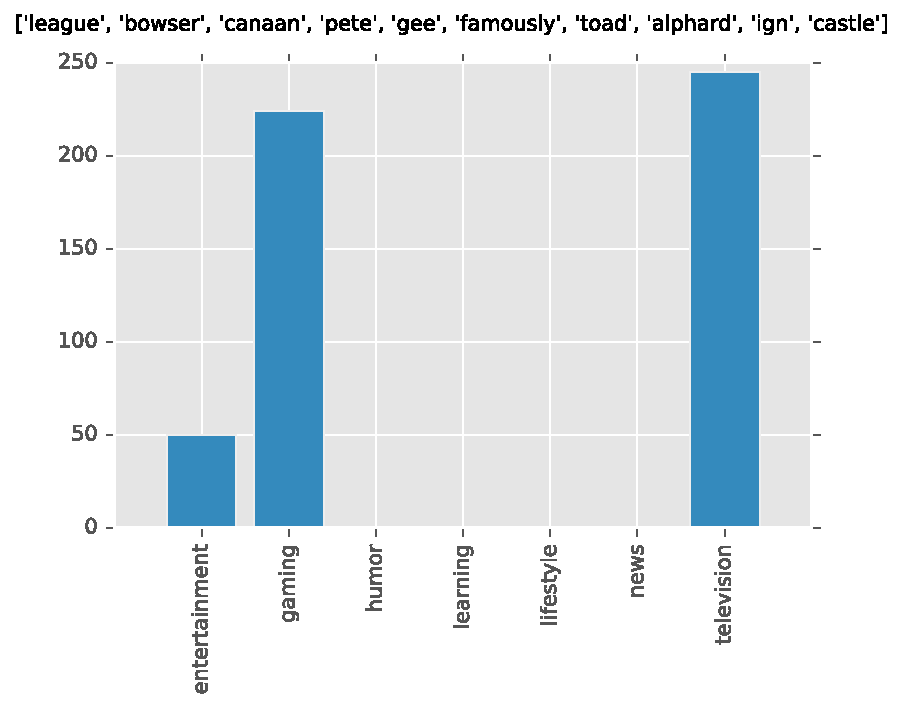
\includegraphics[]{figures/reddit-league-3.pdf}
\caption{``league'' sense 4}
\label{fig-reddit-league-3}
\end{subfigure}
\begin{subfigure}[t]{.3\textwidth}
\centering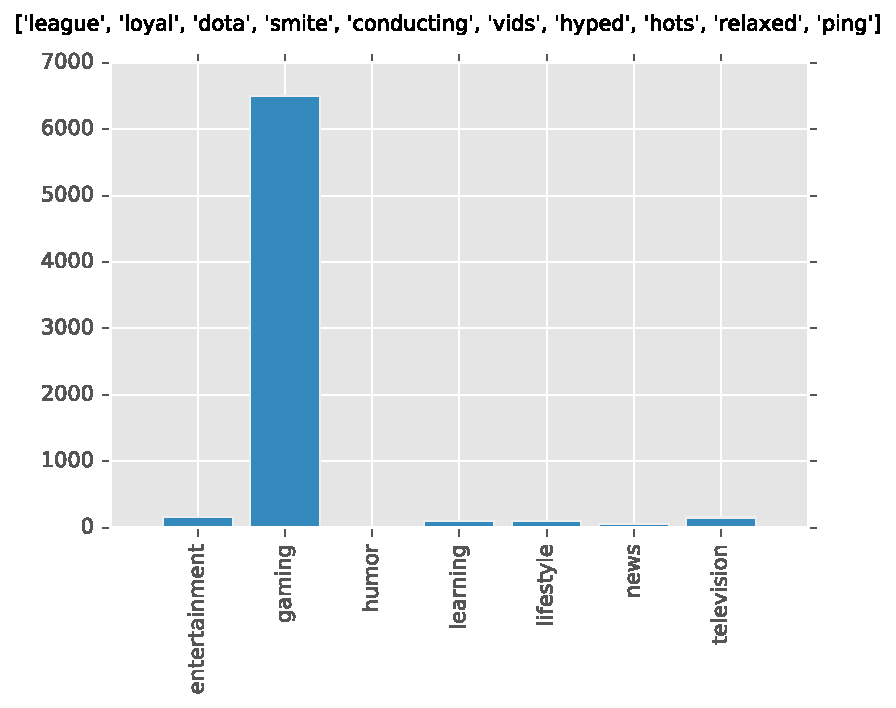
\includegraphics[]{figures/reddit-league-4.pdf}
\caption{``league'' sense 5}
\label{fig-reddit-league-4}
\end{subfigure}
\begin{subfigure}[t]{.3\textwidth}
\centering\includegraphics[]{figures/reddit-league-5.pdf}
\caption{``league'' sense 6}
\label{fig-reddit-league-5}
\end{subfigure}
\begin{subfigure}[t]{.3\textwidth}
\centering\includegraphics[]{figures/reddit-league-6.pdf}
\caption{``league'' sense 1}
\label{fig-reddit-league-7}
\end{subfigure}
\caption{The different senses of the word ``league'' together with the words most similar to the particular sense of ``league''.}
\label{fig-reddit-league} 
\end{figure}

\end{landscape}

\subsection{Identifying Community Word Usage using the MSSG Algorithm}

I test this histogram output on the reference Reddit corpus to see how users in different communities of Reddit use certain words.

Figure \ref{fig-reddit-dark-1} shows a ``dark'' being used in the context of science as in dark matter and dark energy. This sense appears predominantly in the \emph{learning} community which makes sense since this is the community that concerns itself with such topics. Figure \ref{fig-reddit-dark-2} shows ``dark'' being used in the context of the film / story Harry Potter as in dark wizards and dark lord. This predominantly appears in \emph{entertainment} and minorly so in \emph{television}, which again corresponds to intuition. Figure \ref{fig-reddit-dark-4} shows ``dark'' being used in the context of Pokemons as in ``dark Pokemons'', which is used predominantly in the \emph{gaming} community. Finally, and rather unexpectedly, ``dark'' is also used in the context of rum where it is used to describe dark rum. This is used predominantly in the \emph{lifestyle} community in the Reddit corpus.

It was similarly able to distinguish between ``league'' as used in sports and ``league'' as used in gaming (as in League of Legends) as shown in Figure \ref{fig-reddit-league}.

My algorithm adds on to \cite{neelakantan2015efficient} by allowing users to trace the source of the senses of words. This has the following applications:

\begin{itemize}
\item In codeword detection, I am now able to detect when different communities of people use a word different from the rest of their peers
\item In an organization, this can also be used to detect departments / groups of individuals that use a word (may not be a codeword) differently. For example, the name of a boss may be used pejoratively in one department and agreeably in another.
\end{itemize}

However, I still needed a method to systemize the detection of codewords from these histograms.

\subsection{Using KL Divergence to Systematically Identify Codewords}

I then used KL divergence to compare each histogram (for each sense of each word in the corpus) against the uniform distribution. The hypothesis is that a word (such as ``hello'') that is disambiguously used by everyone in the organization should have roughly equal chance of occurring in any of the communities (barring especially lopsided sizes of communities within the corpus, such as one single community taking up 90\% of the corpus). Hence, the sense of ``hello'' as in a greeting should have a near uniform distribution as shown in the ``apple'' example earlier.

The result of doing this is positive. The table below lists the KL divergences of each of the senses of the words in the first row in Figure \ref{fig-reddit-kl}.

\begin{table}[H]
\centering
\begin{tabular}{c c c c c}
\toprule
 good & money & people & dark & league \\
\midrule
0.14463918 & 0.00648365 & 0.16257816 & 0.22922427 & 0.71126526 \\
0.52091641 & 0.43071434 & 0.14932918 & 1.62014716 & 1.90541132 \\
0.06240066 & 0.44830668 & 0.20445455 & 1.59789641 & 1.42980752 \\
0.53456988 & 0.24518687 & 0.09279462 & 0.34249047 & 1.00348243 \\
0.07151459 & 0.14681329 & 0.05849862 & 1.54230648 & 1.54250742 \\
0.44972733 & 0.31814621 & 0.7711894 & 0.83141833 & 1.09152749 \\
0.54374559 & 0.74424692 & 0.1302974 & 0.79688892 & 1.71254201 \\
\bottomrule
\end{tabular}
\caption{KL divergence for each of the senses of the words. Words with rather uniform usage (``good'', ``money'', ``people'') have low KL divergences from the uniform distribution for all senses. However, the usages of ``dark'' and ``league'' highlighted earlier all have high KL divergences}
\label{fig-reddit-kl}
\end{table}

Then, selecting codewords would be a matter of selecting a threshold KL divergence.

\begin{figure}[h]
\centering
\includegraphics[width=.5\textwidth]{figures/reddit-community-histo.pdf}
\caption{KL divergence histogram for all words in the reddit corpus. Finding words that are used specially in a community would be to select a threshold KL divergence}
\label{fig-wsj-count}
\end{figure}

Unfortunately, I did not have time to follow through this.


\begin{appendices}
This section details the additional work I did that do not fit within this main body of research.

\section{Reddit Scraper}

I built a \texttt{node.js} asynchronous web scraper for Reddit, currently hosted at \url{https://github.com/linanqiu/omega-red}. The scraper took around two weeks to build, allowing me access to a very nicely partitioned community dataset that is central to this entire research.

\section{GPU Implementation of Word2Vec}

I verified that the existing GPU implementation of Word2Vec produces erroneous results. \url{https://gist.github.com/linanqiu/e967559d535def1e6f5b931e9b580c58}

\section{Clustering Enron Entities}

I also performed clustering analysis on the Enron entity embeddings. \url{https://gist.github.com/linanqiu/92f0a1cee7663de2ef9df4a042ccfe01}. The results of this experiment can be used to label Enron emails with community labels. This result can then be fed into my community histogram model, producing codewords for the Enron corpus.
\end{appendices}

\bibliographystyle{ieeetr}
\bibliography{biblio}

\end{document}